\documentclass[bibtotoc,liststotoc,BCOR5mm,DIV12]{scrbook}

% use this declaration to set specific page margins
%\usepackage[a4paper , lmargin = {2.7cm} , rmargin = {2.9cm} , tmargin = {2.7cm} , bmargin = {4.6cm} ]{geometry}
\usepackage[a4paper]{geometry}

\usepackage[ngerman, english]{babel}
\usepackage{bibgerm}       		% german references
\usepackage[utf8]{inputenc}   % german characters
\usepackage{graphicx} 				% it's recommended to use PDF images but you can use JPG or PNG as well
\usepackage{url}           		% format URLs
\usepackage{hyperref} 				% create hyperlinks
\usepackage{listings, color}	% for source code
\usepackage{subfig}						% two figures next to each other (example: figure 3a), figure 3b)
\usepackage{scrpage2}					% header and footer line

% header and footer line - no header & footer line on pages where a new chapter starts
\pagestyle{scrheadings}
\ofoot[]{\thepage}
\ifoot{Master Thesis, TU Berlin, Fachgebiet Informatik, 2017}

% set path where images are stored
\graphicspath{{./img/}}

%
% der Befehl \hypenation versteht keine Sonderzeichen, also weder �
% noch "a noch \"a. W�rter die derartige Zeichen enthalten m�ssen
% direkt im Text getrennt werden, z.B. W�r\-ter
%
\hyphenation{te-le-com-muni-cation
te-le-com-muni-cation-specific
Te-le-kom-mu-ni-ka-tions-API
al-ler-dings}
 					% use this file to set explicit hyphenations (doesn't seem to work correctly)

\begin{document}
% ---------------------------------------------------------------
\frontmatter
    \thispagestyle{empty}
\begin{center}

\vspace*{0.5cm}
{\LARGE \textbf{Technische Universität Berlin}}

\vspace{0.5cm}

{\large Institut für Telekommunikationssysteme\\[1mm]}
{\large Fachgebiet für Quality Engineering of Open Distributed Systems\\[5mm]}

Fakultät IV\\
Einsteinufer 25\\
10587 Berlin\\
http://www.qds.tu-berlin.de/\\

\vspace*{1cm}


\includegraphics[width=4cm]{tu_logo.jpg}

\vspace*{1.0cm}

{\LARGE Diploma Thesis}\\

\vspace{1.0cm}
{\LARGE \textbf{Design and Implementation}}\\
{\LARGE \textbf{of a Development and Test Automation Platform for HbbTV}}\\
\vspace*{1.0cm}
{\LARGE Christian Bromann}
\\
\vspace*{0.5cm}
Matriculation Number: 359957\\
16.08.2017\\ % 	date of submission
\vspace*{1.0cm}

Supervised by\\
Prof. Dr.-Ing. Ina Schieferdecker\\
\vspace*{0.5cm}
Assistant Supervisor\\
Dipl.-Ing. Louay Bassbouss
\vspace{3cm}


\end{center}

   	\thispagestyle{empty}
    \cleardoublepage

    \thispagestyle{empty}
\vspace*{3cm}


\begin{center}

\includegraphics[width=0.4\textwidth]{fokuspng.png}
\end{center}

\vspace*{0.2cm}

\begin{center}
FOKUS Institute\\
Kaiserin-Augusta-Allee 31\\
10589 Berlin\\
\end{center}
\vspace*{0.5cm}

\noindent This dissertation originated in cooperation with the Fraunhofer Institute for Open Communication Systems (FOKUS).

\vspace*{1cm}
\noindent
First of all I would like to thank Dipl.-Ing. Louay Bassbouss at the Fraunhofer Institute
FOKUS for giving me the opportunity to carry out state of the art research in this field.
\\
\\
Special thanks to Mister X and Mister Y for their guidance. --- Some personel words... ---
\\
\\
Furthermore I would like to thank ...

    \thispagestyle{empty}
    \cleardoublepage

    \newpage

\thispagestyle{empty}

\begin{large}

\vspace*{6cm}

\noindent
I hereby confirm that the present thesis on ''Design and Implementation of a Development and Test Automation Platform for HbbTV'' is solely my own work and that if any text passages or diagrams from books, papers, the Web or other sources have been copied or in any other way used, all references including those found in electronic media have been acknowledged and fully cited.
\vspace{2cm}

\noindent
Berlin, \today

\vspace{3cm}

\hspace*{7cm}%
\dotfill\\
\hspace*{8.5cm}%
\textit{(Signature Christian Bromann)}

\end{large}

    \thispagestyle{empty}
    \cleardoublepage


    % This template is intended to give an introduction of how to write diploma and master thesis at the chair 'Architektur der Vermittlungsknoten' of the Technische Universität Berlin. Please don't use the term 'Technical University' in your thesis because this is a proper name.
%
% On the one hand this PDF should give a guidance to people who will soon start to write their thesis. The overall structure is explained by examples. On the other hand this text is provided as a collection of LaTeX files that can be used as a template for a new thesis. Feel free to edit the design.
%
% It is highly recommended to write your thesis with LaTeX. I prefer to use Miktex in combination with TeXnicCenter (both freeware) but you can use any other LaTeX software as well. For managing the references I use the open-source tool jabref. For diagrams and graphs I tend to use MS Visio with PDF plugin. Images look much better when saved as vector images. For logos and 'external' images use JPG or PNG. In your thesis you should try to explain as much as possible with the help of images.
%
% The abstract is the most important part of your thesis. Take your time to write it as good as possible. Abstract should have no more than one page. It is normal to rewrite the abstract again and again, so  probaly you won't write the final abstract before the last week of due-date. Before submitting your thesis you should give at least the abstract, the introduction and the conclusion to a native english speaker. It is likely that almost no one will read your thesis as a whole but most people will read the abstract, the introduction and the conclusion.
%
% Start with some introductionary lines, followed by some words why your topic is relevant and why your solution is needed concluding with 'what I have done'. Don't use too many buzzwords. The abstract may also be read by people who are not familiar with your topic.

\thispagestyle{empty}
\vspace*{1.0cm}

\begin{center}
    \textbf{Abstract}
\end{center}

\vspace*{0.5cm}

\noindent

Hybrid Broadcast Broadband TV is one of the latest big developments in the TV industry. It is an effort to standardize the delivery of user-friendly enhanced TV services to the end consumer through connected Smart TVs and set-top boxes. As the standard evolves, it gets rolled out to more countries in the world. With more devices being equipped with this technology, a larger audience is getting access to it which opens interesting opportunities for broadcasters to create new revenue streams via advertisement or pay-TV platforms. Due to the increasing number of manufactures and device models in the market the support level is highly fragmented and aggravates the development of HbbTV applications. To ensure the functionality on a majority of devices a cumbersome and manual testing process is required which is opposed to current standards in software development. The software industry has shifted over the last 5 years from a milestone oriented to an agile approach where shipping qualitative software fast and iteratively is the number one principle. To establish a high development velocity a key factor for success is a solid continuous delivery pipeline that tests software in an automated fashion and provides confidence in the quality of the product.

The major objective of this study is to improve the process of building HbbTV applications by implementing a developing and automation platform that helps HbbTV developers to overcome issues that have been around on web and mobile platforms for years. It examines current standards in debugging and testing of software applications and demonstrates how applying these best practices to the TV space helps to increase the development velocity and software quality of HbbTV applications. By building a debugging bridge that supports the Chrome DevTools Protocol it allows developers for the first time to inspect HbbTV applications in-depth and live on the TV using modern web authoring tools like Chrome DevTools. Furthermore shows this thesis how an Appium automation driver can use this bridge to run functional tests on real Smart TVs in an automated fashion based on the WebDriver protocol.

With that technology in place results demonstrate how powerful debugging HbbTV applications can be and how much information a developer can receive. From the full DOM tree to a JavaScript console up to a detailed report about all received network packages, the state of the app is accessible at any given point in time. Moreover, proves the new HbbTV driver that running automated tests in a continuous delivery pipeline using a tool like Jenkins is fast, reliable and interoperable. A comparison at the end reveals that this approach provides a higher scaleability, functionality and flexibility for debugging and automated testing than any other existing solution in the market before.

    \thispagestyle{empty}
    \cleardoublepage

    % Da die meisten Leuten an der TU deutsch als Muttersprache haben, empfiehlt es sich, das
% Abstract zusätzlich auch in deutsch zu schreiben. Man kann es auch nur auf deutsch
% schreiben und anschließend einem Englisch-Muttersprachler zur Übersetzung geben.

\thispagestyle{empty}
\vspace*{0.2cm}

\begin{center}
    \textbf{Zusammenfassung}
\end{center}

\vspace*{0.2cm}

\noindent

Hybrid Broadcast Broadband TV ist einer der letzten größeren Entwicklungen auf dem Fernsehmarkt. Es ist ein Versuch, über die mit dem Internet verbundenen Fernseh- geräte oder Set-Top Boxen, benutzerfreundliche und erweiternde Sendeangebot an den Zuschauer zu vermitteln. Während sich der Standard weiterentwickelt, wird er bereits in immer mehr Ländern in der Welt bereitgestellt. So erhalten mehr Zuschauer Zugang zu den dargebotenen Services, die für Fernsehsender neue Vertriebsmöglichkeiten, wie Werbung oder Bezahlfernsehen, bieten. Wegen der großen Menge an TV-Herstellern und Modellen ist die Unterstützung der Geräte für HbbTV jedoch sehr unterschiedlich, was die Entwicklung von derartigen Anwendungen deutlich erschwert. Um sicherzustellen, dass diese dennoch auf den meisten Geräten funktionieren, ist häufig ein mühsehliger und manueller Testprozess notwendig. Dies ist mit heutigen Entwicklungsstandards allerdings nicht mehr vereinnehmbar. Die Software Industrie hat sich über die letzten 5 Jahre von einem wasserfall-getriebenen Modell zu einem mehr agilen Anzatz bewegt, bei der kontinuierliche Verbesserungen in kleinen Schritten eines der obersten Prinzipien ist.

Das Hauptziel dieser Master Arbeit ist es, den Entwicklungs- und Testprozess von HbbTV Applikationen zu verbessern, indem eine Plattform geschaffen wird, die HbbTV Entwicklern hilft, die selben Probleme, die es bereits für Web- und mobile Anwendungen seit Jahren gibt, zu lösen. Sie untersucht die aktuellen Standards in der Entwicklung und Qualitätssicherung von Software und zeigt auf, wie diese Methoden ebenfalls im Bereich des Fernsehens angewendet werden können. Indem ein Kommunikationskanal zwischen Applikation und modernen Entwicklungsanwendungen, wie z.B. den Chrome DevTools, geschaffen wird, ermöglicht diese Arbeit Entwicklern zum ersten Mal, detailierte Informationen über die Anwendung während der Entwicklung in Erfahrung zu bringen. Zudem zeigt sie auf, wie durch die Bereitstellung eines Automatisierungsprogammes, welches diesen Kommunikationskanal nutzt, funktionale Tests auf echten Fernsehgeräten ausgeführt werden können.

Durch diese Technologien wird demonstriert, wie effizient die Entwicklung von HbbTV Anwendungen sein kann. Der Entwickler erhählt, neben dem Applikationsaufbau, einer JavaScript Konsole und einer detailierten Auflistung aller Netzwerk Pakete, nicht nur umfangreiche Information über die Applikation an sich, sondern auch über ihren Zustand zu jedem beliebigen Zeitpunkt. Zudem beweist das Automatisierungsprogramm wie schnell, zuverlässig und vielseitig funktionale Tests in einem automatisierten Prozess, z.B. durch die Nutzung von Programmen wie Jenkins, ausgeführt werden können. Im Vergleich am Ende wird bewiesen, dass dieser Ansatz für die Entwicklung von HbbTV Anwendungen weitaus besser skalierbar, funktionaler und flexibler ist als jegliche bereits existierende Lösung auf dem Markt.

    \thispagestyle{empty}


    \tableofcontents
    \thispagestyle{empty}

    \listoffigures
    \thispagestyle{empty}

    \listoftables
    \thispagestyle{empty}

% --------------------------------------------------------------

\mainmatter % comment single chapters for faster compilation

    \chapter{Introduction\label{cha:introduction}}

In the late 19th century a Germand student named Paul Gottlieb Nipkow developed an electronical device
that was able to send images over the wire with the help of a rotating metal disk. This was one of the first
mechanical prototypes that suppose to become the television. With the beginning of the 20th century two types
of TVs emerged: mechanical and electronic television. Even though the mechanical type has seen a lot of
innovation by 1934, all television systems had been converted to electronic machines. These became more and
more popular in humans households so that almost 10 years later the number of U.S. homes with television sets
could be measured in the thousands and by the late 1990s more than 98\% of U.S. homes had at least one
television. The device was one of the first electronic devices that introduced a new generation of entertainment
human equiment that everyone suppose to have.\\
Despites innovations like colored displays or flat screen devices the television quickly lost the race against
the mobile phone as well as the personal computer and later laptop. Even though it is still a very popular
medium, people nowadays use their smart phone or personal computer way more frequent as it was at the end of the
20th century. One of the major reasons was the innovation of the internet. The more people were able to connect
each other and consum media over the world wide web the more became the television the less frequent choice.
The new generation of kids grows up with web media portals like YouTube\footnote{\url{https://www.youtube.com/}}
and generates billions and billions of clicks, views and revenue for advertisment companies every day.\\
Thanks to the most recent big innovations in television technology that are setup boxes and standards like
Hybrid Broadcast Broadband (short for HbbTV) the TV industries tries to keep up with other technologies by
introducing the so called smart televisions or sometimes referred to as connected TV or hybrid televisions.
It is the first generation of such devices that are connected to the world wide web and therefor can provide
digital content in a non linear way for the first time.\\
Since then the market and the amount of smart TVs has been growing fast. With that the HbbTV standared evolved
and more and more broadcaster have build an app for their broadcast streams. World wide have more than 25
countries (mainly in Europe) adopted the standard and broadcaster have developed around 300 apps that can
be viewed by more than 43 million sold devices with HbbTV support\footnote{\url{https://www.hbbtv.org/news-events/hbbtv-ibc-2016-services-and-devices/}}.
Numbers are growing. It shows the tremendous potential of the market and the beginning of a paradigm shift
from linear TV stream to non linear media content ondemand.

\section{Motivation\label{sec:motivation}}

By introducing TVs to the Internet it automatically opened the door for web technologies to become standards
on these devices. While early setup boxes like Chromecast\footnote{\url{https://www.google.com/intl/de_de/chromecast/}}
enabled some web-browsing experience, HbbTV has been the first real technology that brought websites to the big screen.
Instead of just watching a stream with linear content, HbbTV supported devices also provide web sources that
contextually fits to the viewed content and allow the user to navigate through an app to watch non linera content
ondemand.\\
These apps are webpages with JavaScript heavy functionality that are rendered in proparitary browsers. Unlike
normal browsers though there is no navigation menu or status bar. The page is rendered with a transparent background
so that you can show the TV stream in the back while navigating through the app. Depending on the TV manufacture
the embedded browser in the TV is mostly a clone to the existing desktop browsers though with less compatibility.
Early HbbTV supported devices are compatible with desktop browsers that have been shipped more than 10 years ago.
Especially since HbbTV runs a lot of JavaScript to show its content in a dynamic way this makes it hard for
developers to build their apps.\\
Compared to modern web development where almost everything is made out of web components, build together in a
modular fashion using tools like React, Polymer or Angular, HbbTV apps are still build like JavaScript single
page applications from 10 years ago. Not only because the technology within the browser doesn't allow to use
latest web technologies also the developer integration with common used tools on the developers machine is due
to device boundaries not possible. Since the internet is around way longer than the fact that it is supported on
TV devices the process of web development has become an own industry and tooling around it an own market.
Companies constantly build frameworks, tools and integrations that makes building complex web apps easier and
maintainable. Especially browser vendors like Google or Mozilla are interested in providing an excellent
developing experiences as this has become the only differentiator between browsers these days. After web
technologies has been standardised by the W3 Consortium\footnote{e.g. latest HTML specification: \url{https://www.w3.org/TR/html5/}}
the compatition between browsers is not based on the question who can interpret the HTML code better and therefor
render the page more correctly but more on which browser supports the latest recommended standards and fanciest
technologies.\\
Unfortunatelly this is not the case for all embedded browser in smart TVs. The HbbTV standard was developed as
a superset of HTML and JavaScript. The specification itself recommends support for certain APIs but doesn't
require the manufacture to embed the latest browser and all their features. This is partially due to the fact
that not all web technologies are applicable on a television. For example there is no WebRTC support because
most of the TVs don't have a camera installed. Also an HbbTV application was suppose to only add contextual
information to the provided broadcast stream. Building complex web applications was never considered to become
realitiy at the first place. However as more broadcaster discovered the opportunities that HbbTV can bring to
the audience more people were interested in finding new ways to deliver interactive content to everyone in
front of the screen.\\
This yields a problem that has been around in web development for ages but almost died due to the standardisation
of web technology. With more support for the HbbTV standard the manufacture started to improve the functionaility
of embedded browser not only by adding more computing power to smart TVs but also by providing better compatibility
to already accepted web standards. In addition to that the HbbTV standard itself evolved and requires now certain
technology to be supported in order to allow the TV to label itself as HbbTV compliant. The problem with this is
that not everyone buys a new TV as soon as there is a better one on the market. Especially since they last longer
than usual mobile phones or computer the update cycles of televisions are long. Compared to desktop browser which
update themself automatically and have reached version numbers in the fifties, the browser within todays smart
TVs don't update and stick as long as the owner keeps the television. This creates a highly fragmented
user market with tons of different devices over time that all support a different level of HTML and JavaScript.
Building qualitiv HbbTV apps that suppose to run on the majority of devices in peoples households becomes super
time consuming and expensive since you don't know if the device can execute your scripts or if you've used
functionality that is not supported. As a developer you not only have to have all the TV devices which is literally
impossible but you also need to manually test your app on each one of these. This process is cumbersome and not
scaleable.

\section{Objective\label{sec:objective}}

With the HbbTV standard not being older as a couple of years the development and quality ensurance process for
building apps for the smart TV is lagging behind modern web development standards. Due to the high fragmentation
of televisions on the market it is almost impossible to ensure 100\% functionality for each individual TV.
In addition to that since the browser that renders the app is embedded on a remote device it appears to be
way more difficult to not only build HbbTV applications but also to debug them in case a certain TV doesn't
run a certain functionality. In addition to that since HbbTV is a fairly new standard on the market it has not
even closed developed a community around the technology compared to the modern web on desktop and mobile. Not
more than a handful frameworks has been developed so far that can simplify the work of an HbbTV app developer. Most
of the problems still have to be solved individually which increases the probability of introducing errors and
issues that have to be fixed.\\
The goal of this thesis is to mitigate common developer issues when building HbbTV applications for arbitrary
Smart TVs by providing a set of tools that has been proven to be useful for modern web development on desktop
and mobile. The way how we build apps should not be any different when switching between computer, handheld or
television devices. Due to standardisation and integration work that has been done so far we gathered a relieable
set of tools that work perfectly with each other and is known by every developer. Current HbbTV app development
is extremly painful when it comes to debugging and web-authoring. Often people build their home grown solutions
which is not more or less than a panel with logging messages. There is no real interaction happening between app
and app developer. This makes fixing bugs almost a trial and error process.\\
By bringing modern web tooling to the TV we don't only improve dev experience but also increase the velocity
and quality of shipping HbbTV apps to the market. Looking at televisions being no different than other internet
connected devices these days we should try to adapt technologies for quality ensurance like automated testing
approaches to improve the way we test HbbTV apps. Especially since the mobile market is similar fragmanted
than the TV market we should take a look at how mobile solved this problem and try similar approaches to solve
it. Ultimately the developer should not care about whether he is testing a desktop, mobile or HbbTV app. All
he needs to know is the app itself and the features he wants to test, the rest should be identical to any other
app or websites he builds.

\section{Scope\label{sec:scope}}

As the title of this thesis discloses I will try to design and implement a development and test automation
platform for HbbTV based applications. We should look sepetately on these objectives as they fulfill different
purposes for the developer.\\
The development platform should provide HbbTV app developer a way to debug and interact with the app on the
TV in a similar fashion than he would do on the desktop using his favorite browser. Recent browser statistics
\footnote{Browser statistics is hard to measure and always depends which user base you track. However regardless
if you look at more general statistic like StatCounter (\url{http://gs.statcounter.com/}) or a more web developer
oriented one like W3Schools (\url{https://www.w3schools.com/browsers/}) it shows that Google Chrome has by far
the biggest market share world wide.} clearly show that Google Chrome is not only the most used browser in the
market but also the most prefered browser for web development. The main reason is its built in Chrome Developer
Tools\footnote{\url{https://developer.chrome.com/devtools}} that \textit{''give[s] developers access to the internal
workings of the web browser and web apps''} \cite{devtools}. Since it is so popular and well known to developers
I will find and implement a way to use Chrome's Devtools application to debug HbbTV apps directly on a smart TV.
The Devtools app itself is nothing more than a usual web app that can be used by the Chrome browser. It is
publicly available on GitHub\footnote{\url{https://github.com/ChromeDevTools/devtools-frontend}} and can be used
with respect of Googles license agreement\footnote{\url{https://github.com/ChromeDevTools/devtools-frontend/blob/master/LICENSE}}.
That being said, the actual technical work here is not to rebuild the Devtools application but to reverse
engineer the communication that happens between that app and the browser in order to enable information exchange
and debugging commands. Due to the fact that the browser that renders an HbbTV app on the TV does not disclose
these information we need to find a way to provide these by injecting a script that can send us all the details
of the HbbTV app based on the \textit{''Chrome DevTools Protocol''} \cite{devtoolsprotocol}. Due to limitations
in time, implementation and technical support of the browser that is running on the TV it won't be possible to
support all features that the DevTools app provides. The work concentrates only on parts that are relevant to
an HbbTV app developers interest and which are feasible with all the limitiations of the browser on the TV.
To be more specific, the developer will be able to see the DOM structure of the app as well as its sources and
network traffic. He will be able to change attributes of DOM nodes and remove them. In addition to that he will
be able to use the console tab to run arbitrary JavaScript code getting executed on the TV in the same runtime
environment as the app. With that the developer will be able to access the global scope of the runtime and therefor
also inspect certain states of the app. There will be two different ways provided to inject the script that
enables the communication with the DevTools application.\\
Based on this work the test automation platform will allow to run automated tests using the Webdriver protocol
\footnote{\url{https://www.w3.org/TR/webdriver/}} on real TV devices in the lab. As foundation I will build the
test automation driver based on Appium's base driver. Appium is a framework for mobile test automation and home
for a lot of drivers that allow us to run automated tests on iOS, Android, Mac OS and even Windows applications.
Using a Raspberry Pi as automation proxy I will equip TVs in the lab to run that automation driver and connect
it to a Selenium Grid server in order to run Selenium tests in any programming language and with any framework
that supports the latest Webdriver protocol. Using continuous integration and delivery (short CI/CD) tools like
Jenkins\footnote{\url{https://jenkins.io/}} we will hook up an actual HbbTV app that will be tested on different
TVs everytime someone changes the code in the repository. With the help of various test reporters we will be then
able to indentify issues that come up during testing to spot bugs that had been introduced by the developer
imitately. Since the Webdriver protocol is specialised for browser automation some of its specifications won't
apply for TV devices. As the only input device for televisions so far is the remote control the test driver won't
cover the whole protocol. User prompts, element interactions like click and keyboard actions are not designed
to work on a TV. Also due to time limitations I will not cover screen capturing or frame switching as they are
not important commands to ensure the quality of HbbTV apps.

\begin{figure}[htb]
  \centering
  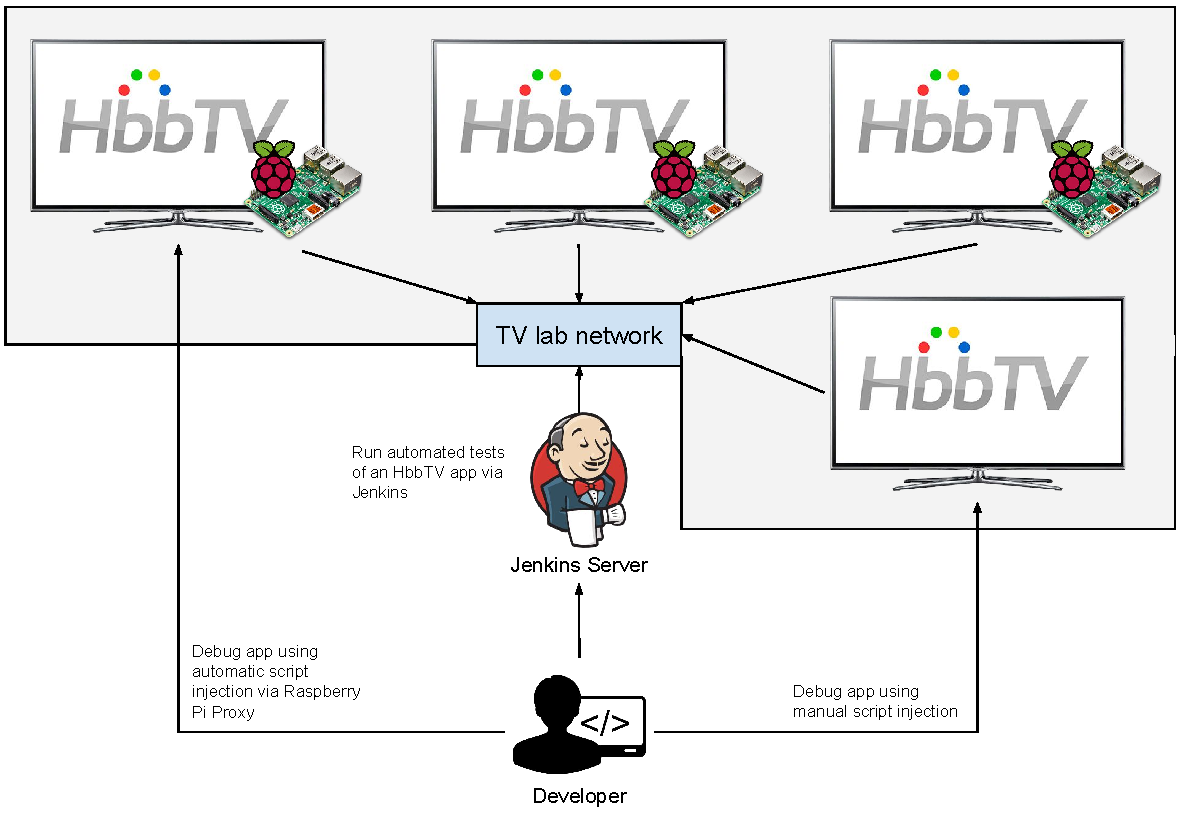
\includegraphics[width=15cm]{big_picture.pdf}\\
  \caption{Big picture of how developers will be able to develop and test their HbbTV application}\label{fig:bigpicture}
\end{figure}

With both platforms in place the developer of an HbbTV app will be able to debug and test his applications
with modern tooling that is used in todays web development. Since the technologies for both is based on
common used and well defined standards we don't restrict ourself to another home grown solution instead we
allow the integration to other tooling which makes us less bound to a certain tool. As described in Figure
\ref{fig:bigpicture} the developer will have three different ways to utilize the TV. One way is to use
a TV that was equipped with a Raspberry Pi running the automation driver on it. The Pi will act as a proxy
and allows to automatically inject the automation script as well as track network data to display it in the
DevTools. Because of the amount of edge cases and issues this proxy can run into there will be no guarantee
that this approach is a bullet proof and easy to use solution. Running this kind of setup requires some amount
of effort to maintain it. That's why there will be another way to debug and test HbbTV apps without a
Raspberry PI. This solution will require some manual changes to the source code of the app to make it work.
To demonstrate the flexibility of the debuging and testing platform I will showcase at the end a common
CI/CD workflow to run automated tests on a real HbbTV app.

\section{Outline\label{sec:outline}}

The 'structure' or 'outline' section gives a brief introduction into the main chapters of
your work. Write 2-5 lines about each chapter. Usually diploma thesis are separated into
6-8 main chapters.\\
\\
\textbf{Chapter \ref{cha:chapter2}} is usually termed 'Related Work', 'State of the Art'
or 'Fundamentals'. Here you will describe relevant technologies and standards related
to your topic. What did other scientists propose regarding your topic? This chapter makes
about 20-30 percent of the complete thesis.\\
\\
\textbf{Chapter \ref{cha:chapter3}} analyzes the requirements for your component. This
chapter will have 5-10 pages.\\
\\
\textbf{Chapter \ref{cha:chapter4}} is usually termed 'Concept', 'Design' or 'Model'.
Here you describe your approach, give a high-level description to the architectural
structure and to the single components that your solution consists of. Use structured
images and UML diagrams for explanation. This chapter will have a volume of 20-30
percent of your thesis.\\
\\
\textbf{Chapter \ref{cha:chapter5}} describes the implementation part of your work. Don't
explain every code detail but emphasize important aspects of your implementation. This
chapter will have a volume of 15-20 percent of your thesis.\\
\\
\textbf{Chapter \ref{cha:chapter6}} is usually termed 'Evaluation' or 'Validation'. How
did you test it? In which environment? How does it scale? Measurements, tests, screenshots.
This chapter will have a volume of 10-15 percent of your thesis.\\
\\
\textbf{Chapter \ref{cha:chapter7}} summarizes the thesis, describes the problems that
occurred and gives an outlook about future work. Should have about 4-6 pages.

    % Chapter 2 is usually termed 'Related Work', 'State of the Art' or 'Fundamentals'. Here you will describe
% relevant technologies and standards related to your topic. What did other scientists propose regarding
% your topic? This chapter makes about 20-30 percent of the complete thesis.
%
% This section is intended to give an introduction about relevant terms, technologies
% and standards in the field of X. You do not have to explain common technologies such
% as HTML or XML.
%
% This section describes relevant technologies, starting with X followed by Y, concluding with Z.

\chapter{State of the Art\label{cha:state_of_the_art}}

There are literally two main standards/protocols that are used in this thesis and will be described in
depth in this chapter: the HbbTV standard and the Webdriver protocol. Both are fairly new standards that
have been defined within the last 5 years. Another important protocol for this work is the Chrome Remote
Debugging protocol which is used by the automation driver to drive the Webdriver tests get data out of
the HbbTV app. This thesis tries to connect the standards to allow interoperability between them to
increase the level of integration to a wide variety of tools that has not been possible before.

\section{HbbTV\label{sec:hbbtv}}

% It's always a good idea to explain a technology or a system with a citation of a prominent
% source, such as a widely accepted technical book or a famous person or organization.

Television devices started to become connected to the internet already before HbbTV was invented. With
the so called Set Top Boxes or Smart TV Sticks customers were able to connect the TV to an internet
capable device that provided a content stream. Big companies like Google, Amazon or Apple provided such
devices. The problem with this approach was that if a developer wanted to build an app he had to create
this app for each individual platform. This is a really time consuming and not scaleable process as
the way you build apps for such platforms was extremely different. After game consoles like Sony Playstation
or Microsofts xBox became internet connected devices too there even was another way to transform
the normal TV to a Smart TV. It made it even more difficult for content provider to deploy their services
to all TV platforms.

With the open ETSI standard called HbbTV a new way was build to create digital applications for
broadcaster and content provider that runs on every TV supporting that standard. It \textit{''is
a globally initiative technology mainly developed by industry leaders''} \cite{zte}. The standard
itself introduces only a handful technical components and is mainly based on existing standards. HbbTV
applications are HTML webpages with additional features that enable certain interaction between
broadcast and broadband. It is sometimes referred to as Hybrid Television since the TV device receives
data from both of these sources in parallel. This means that from a running broadcast stream it allows
customers to open apps that provide additional content to the image on the screen. From that you can start
even more applications that provide different content in non linera fashion. We have to differentiate
here between two different types of apps. There are broadcast-independent applications that are not
connected to any broadcast service and are downloaded and accessed via broadband. The other type are
broadcast-related applications that can be opened when a certain broadcast service is used. They
can start automatically or explicitly upon user request. The advantage of HbbTV here is the independence
to the used device. Content provider can build and deploy apps which can be used by any device if the
standard is supported.

If a consumer is equipped with an HbbTV supported Smart TV he will usually see a small image somewhere
on the screen that asks him to press the red button on the remote control. Pressing it triggers an
event within the app that opens the HbbTV application. Once the user switches the channel the same
happens again with a different app. Depending on the broadcaster each broadcast signal contains
a small AIT package that contains main information like application ID, version, autostart state and
application URL of the HbbTV app. Figure \ref{fig:app_delivery} demonstrates the workflow of this
process.

\begin{figure}[htb]
  \centering
  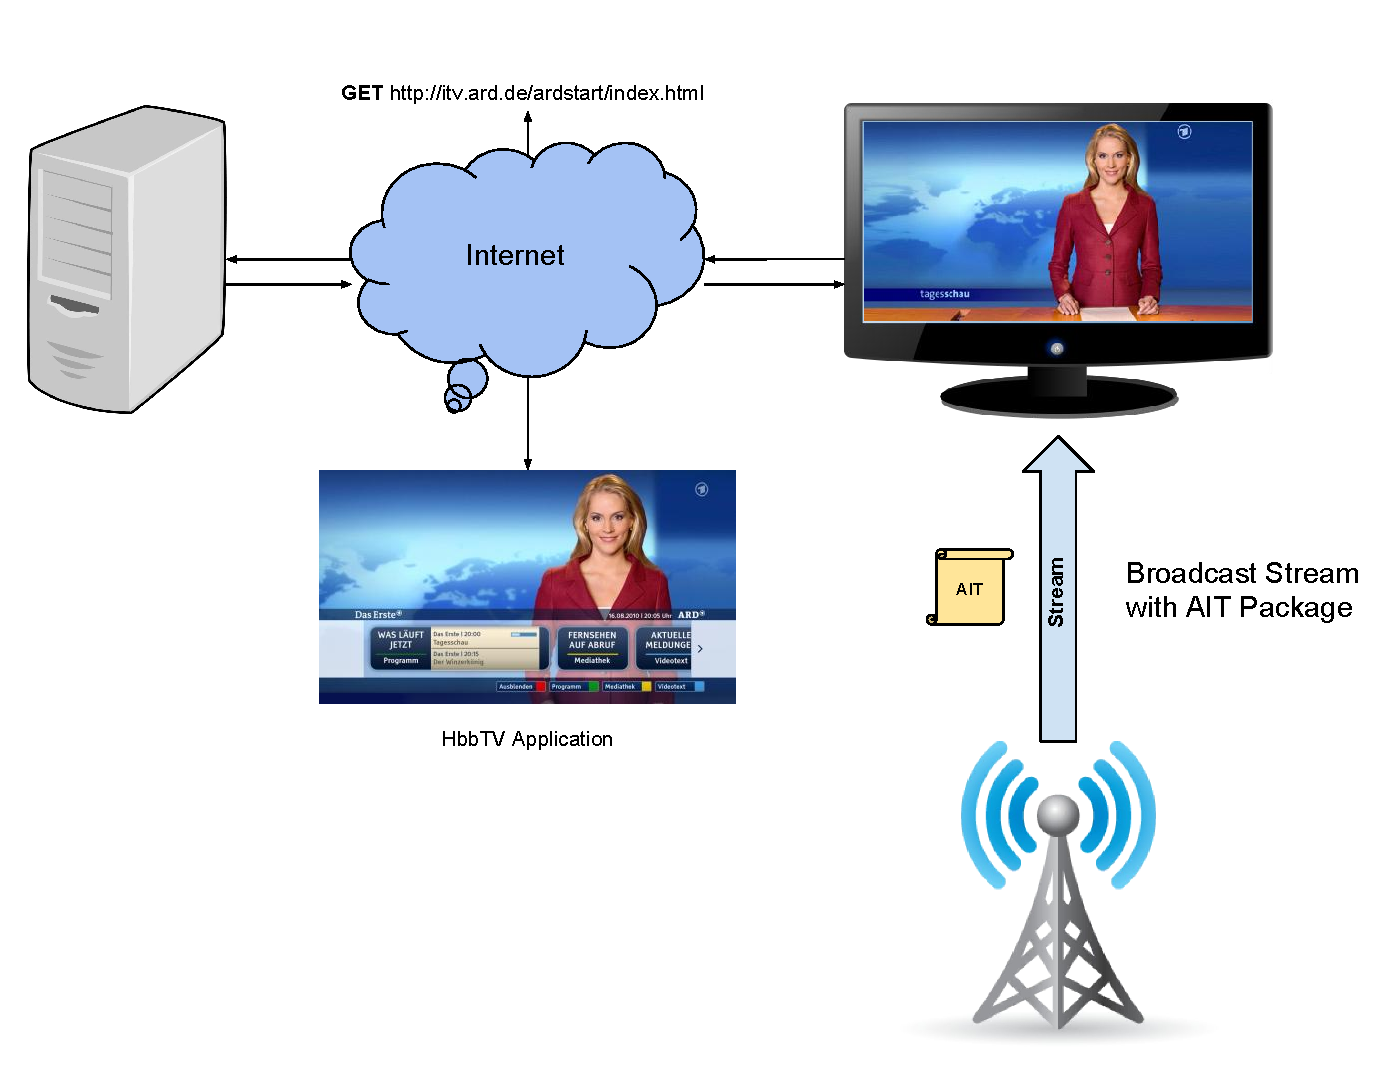
\includegraphics[width=15cm]{app_delivery.pdf}\\
  \caption{App delivery workflow of HbbTV applications}\label{fig:app_delivery}
\end{figure}

Depending on the autostart information within the AIT package the app either starts automatically
as soon as the broadcast stream starts or only when the user pushes the red button. Most HbbTV
applications these days use the autostart feature to display a small indicaticator image to
show that an HbbTV app is available to use. Once the app opens it either takes up only some part
of the screen fulfills the whole display. In general though the broadcast stream is never
getting disrupted as the application only acts as an additional service to the broadcast stream.

After the first specification was released in 2010 by the \textit{''HbbTV forum and published by ETSI
in the specification TS 102 796''} \cite{evolution} initiators reached out to CE manufactures to get
it implemented in the next generation of TVs. Since then the number of Smart TVs with HbbTV support
increased drastically with more than 43 million devices sold and over 300 apps deployed in 25
countries\footnote{Source: \url{https://www.hbbtv.org/news-events/hbbtv-ibc-2016-services-and-devices/}}
\footnote{A complete list of all countries can be found in Listing \ref{hbbtvdeployed} in the annex section}.
Alone in Germany there are over 120 HbbTV supported channels\footnote{Source: \url{https://trifinite.org/hbbtv/trifinite_hbbtv_channel_list.html}}
generating roughly 320 million hits monthly\footnote{Source: \url{https://goo.gl/eg8Sfs}}.

Almost two years later a new specification was released (HbbTV 1.5) that added support for MPEG DASH
and MPEG CENC. MPEG DASH is an ISO standard for adaptive streaming of IP videos. Depending on the
users bandwith and CPU processing power it ensures continuous playback and helps improving the stream
experience in general by monitoring the CPU utilization and/or buffer status. If e.g. for any reason
the user looses bandwidth the video is able to lower the quality of the video so that it still can
be played without disrupting. Due to support issues not many HbbTV apps use DASH these days.
Most videos are still loaded in a progressiv way. The MPEG CENC on the other side helps with common
encription for ISO base media format files and MPEG-2 transport streams. As content provider using this
feature you only have to encrypt your video once. The user then has to decrypt it by getting the
key from one of many DRM systems.

The HbbTV 1.5 standard is supported by the majority of devices these days however many CE manufactures
already are about to support the latest HbbTV spec version 2 with their new devices on the market.
It introduces a lot of new features and supports more web technology standards. While previous HbbTV
apps only work with a version of CE-HTML which is an XHTML-based standard specifically for consumer
electronic devices on UPnP networks, the latest specification supports HTML5, CSS3 and Web Sockets.
Another new feature is the ability for synchronisation of audio, video and data streams that enables
the consumer to watch a certain broadcast stream while listening on the audio via broadband. This
opens a wide variety of use cases like service for simultan translations to videos. It can be
combined with the new introduced Second Screen Integration for Smart Phones and Tablets which
allows to start broadcast streams from your personal handheld on the TV. Due to its duplex
communication ability it allows to also start videos from your HbbTV app on your mobile device.
This works with multiple devices and also provides a lot of opportunities for e.g. gaming applications
where phones can be used as remote controls. In the video area the specifications will support
new streaming formats like HEVC, also known as H.265 and MPEG-H Part 2, DASH for DVB or
push-on-demand where users are able to download certain videos on a local storage to watch them
if desired.

It is worth mentioning that version 2 of the spec was never really released by ETSI. It got
surpassed by version 2.0.1 which fixed unclear specifications and removed some errors. It also
shipped some additional specifications that were required to adapt the standard in Italy and United
Kingdom who have decided to move from a similar standard called MHP to HbbTV. These specifications
define additional caching rules for HTTP/1.1, more details on higher display resolution and other
technologies that were defined in MHP.

An additional standard to HbbTV was released short after HbbTV version 2 was published by ETSI.
This standard is called Application Discovery over Broadband and is not part of the actual
HbbTV specification. However it adds an important addition to HbbTV when cable service provider block
the AIT of the broadcast stream. These provide have a different idea of interactive TV services
and usually want to promote their own platform. Once the AIT package is blocked the HbbTV application
can't be loaded by the TV anymore since information about application ID and URL are missing.
Application Discovery over Broadband is a workaround to solve this problem.

\begin{figure}[htb]
  \centering
  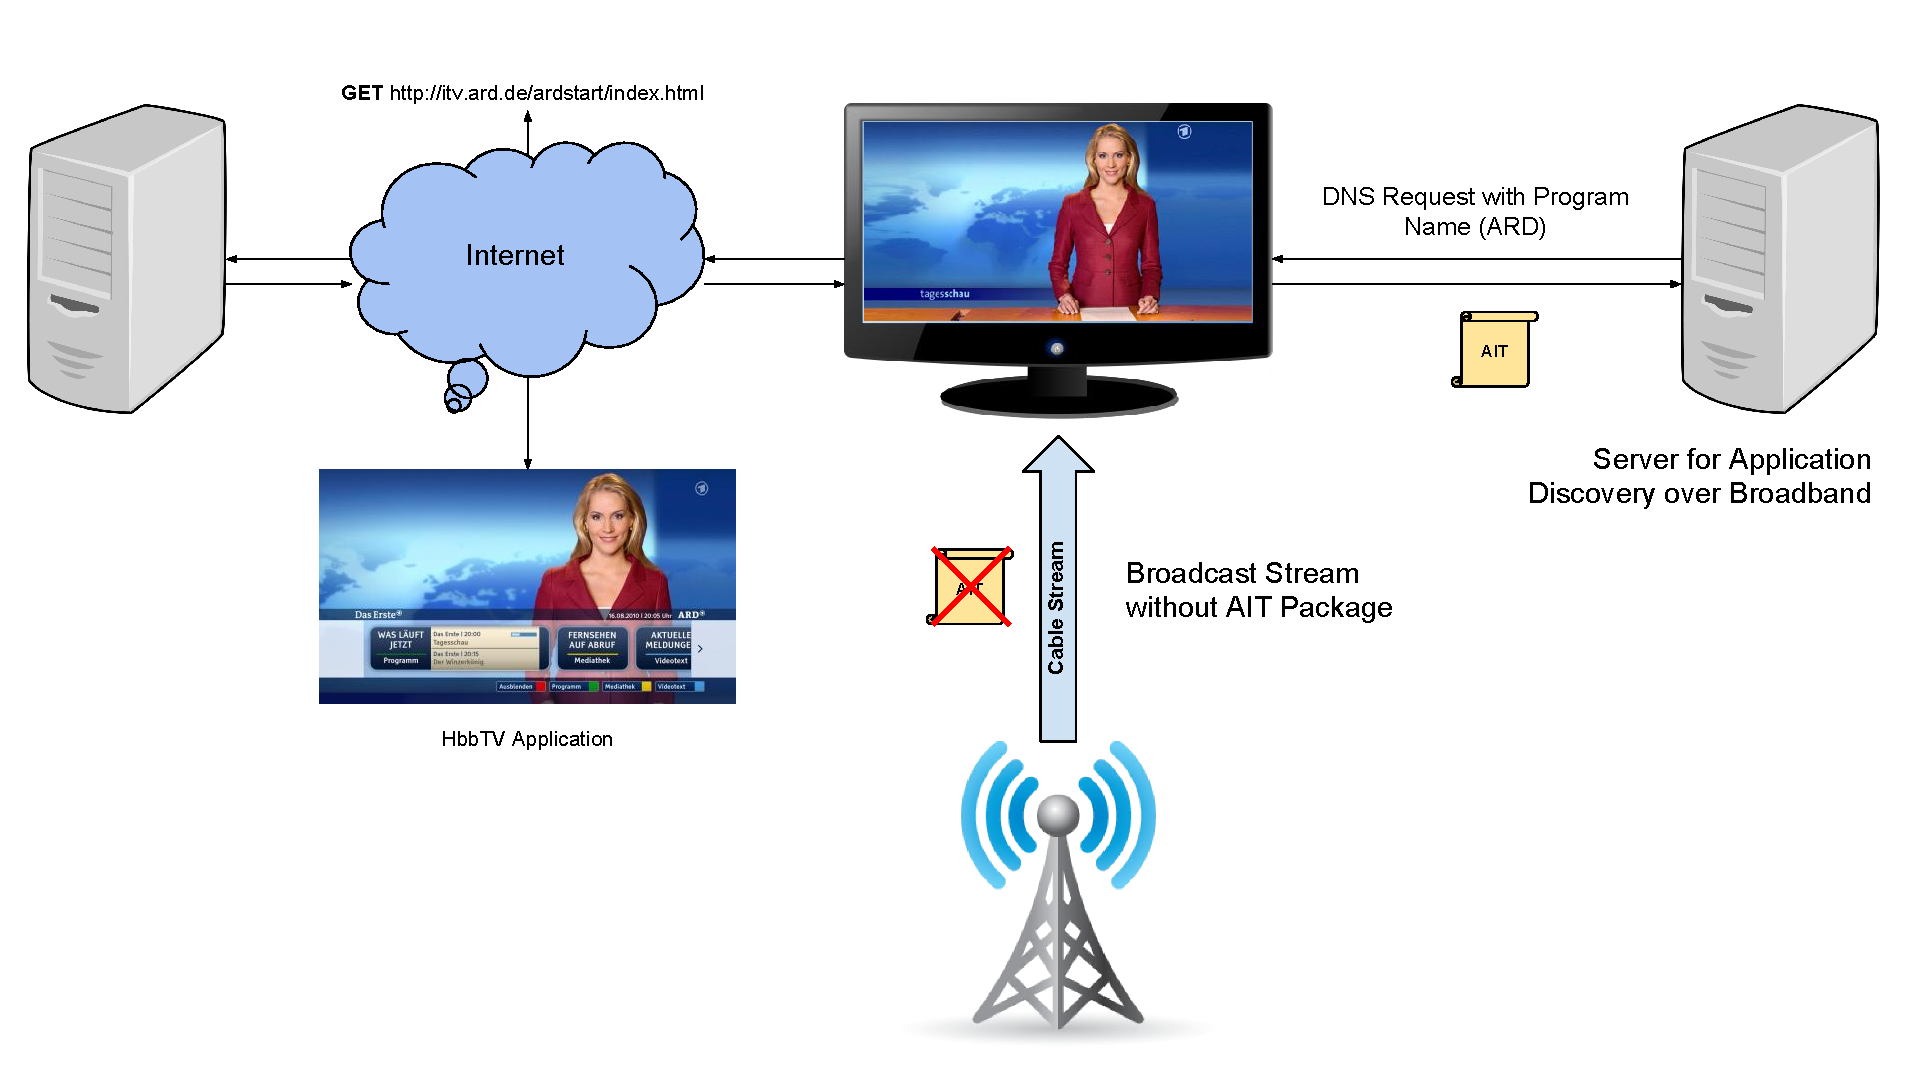
\includegraphics[width=15cm]{application_discovery_over_broadband.pdf}\\
  \caption{App delivery workflow of HbbTV applications over broadband discovery}\label{fig:application_discovery_over_broadband}
\end{figure}

As described in Figure \ref{fig:application_discovery_over_broadband} the TV gets the AIT package
from a dedicated server based on the program name. Each broadcaster usually has their own DNS
root server and an own AIT server. However there is one main HbbTV DNS root server which routes the
DNS request from the TV to the server of the broadcaster.

Pay, cable, IPTV or Sat-Platform operators as mentioned above sometimes provide instead of HbbTV
their own service apps with own GUI. They usually require some sort of additional hardware which
don't support HbbTV. Even though the TV is connected to the internet and supports the standard
it is still not possible to open up an HbbTV application. As solution for this problem the
consortium around the standard invented the so called Operator Apps which allow to connect
operator and HbbTV applications on one Smart TV. The idea is that the user can switch between
both worlds as a functionality within the TV. An operator can become anyone who has a contract
with the TV manufacture. Each operator app has to authenticate to the TV to avoid abuse. Unlike
HbbTV applications and operator app can run in the background at all times and can display
messages on the display as well as overwrite key functions like \textit{''P+''} or \textit{''P-''}.
They open usually by pressing \textit{''EPG''} or \textit{''Menu''}. In the specification of
operator apps which is part of HbbTV verson 2 the consortium emphasized that operator and HbbTV
apps can live seamlessly together.

Looking back at the standard that was first specified 7 ago HbbTV has taken a very interesting
development. From being able to show more than a digital and interactive teletext to supporting
HTML5 and Second Screen it became quite comprehensive. This enables broadcasters to use this
service in a variety of ways.

\subsection{Example Applications And Use Cases}

All these features allow broadcasters to implement not only an additional content outlet but also
to create tailored advertisment strategies to a specified audience. With methods like geotargeting
or targeted advertisment. Geotargeting can be used in HbbTV applications by leveraging a users
IP address in order show regional products or services. Combined with a broadcast stream it
enables interesting opportunities. In an advertisment campaign launched by Germans private
broadcaster RTL they promoted a pharmaceutical with help of an HbbTV app. The pharmaceutical
\textit{''Wick Medinait''} was advertised along with a banner that showed the regional weather
forecast. It had the effect that the HbbTV app banner supported the TV spot so that it increased
the impact of the advertisment itself.

\begin{figure}[htb]
  \centering
  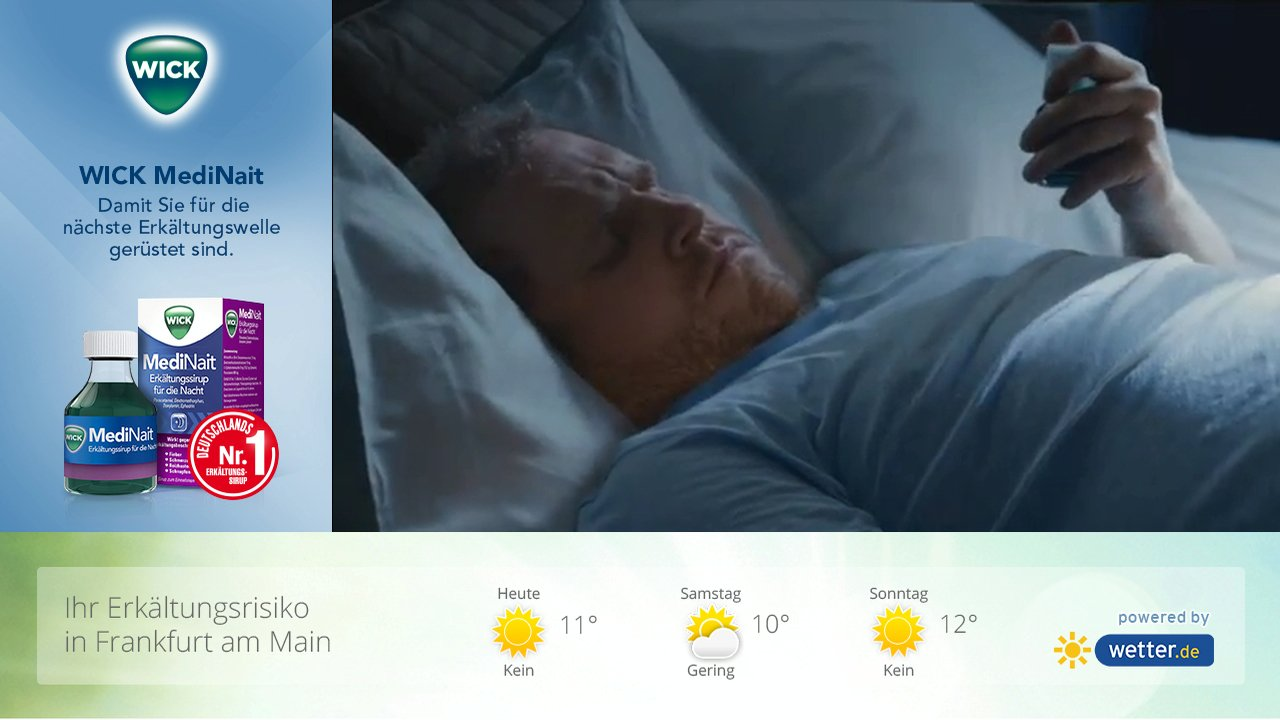
\includegraphics[width=10cm]{geotargeting.jpg}\\
  \caption{
    Use case of geotargeting via HbbTV\\
    {\tiny Image Source: https://goo.gl/rab8XD}
  }
  \label{fig:geotargeting}
\end{figure}

This is also called Addressable TV advertising. It \textit{''enable[s] advertisers to selectively
segment TV audiences and serve different ads or ad pods (groups of ads) within a common program or
navigation screen. Segmentation can occur at geographic, demographic, behavioral and (in some cases)
self-selected individual household levels [...]''}\cite{adrTV}.

Another interesting use case outside of advertisment is content authoring of HbbTV applications.
Usually an HbbTV application is a custom web app that is build to serve a specific content for
a service or show. Once you want to promote a new service or show it requires to build a new
app with new content. This takes time and cost money. A solution to this problem was adapted from
the web. By using a Content Management System (CMS) like Wordpress\footnote{\url{https://wordpress.org/}}
broadcaster can create or modify the content of their apps using a simple web interface.

\begin{figure}[htb]
  \centering
  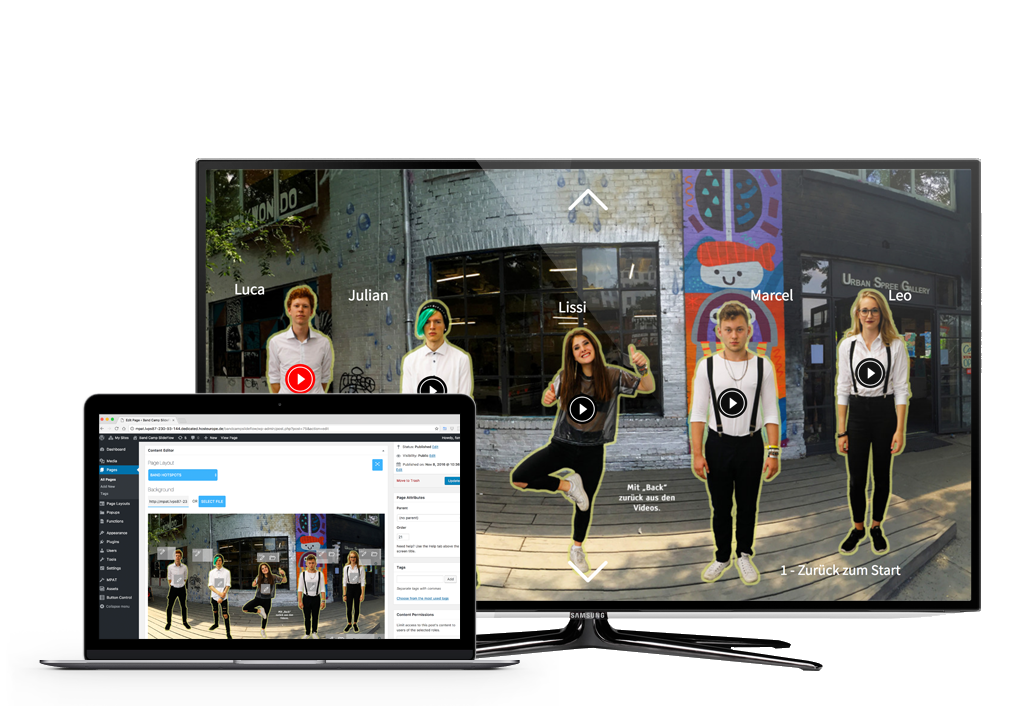
\includegraphics[width=10cm]{mpat.png}\\
  \caption{
    Modifying HbbTV content via a web interface
  }
  \label{fig:mpat}
\end{figure}

Figure \ref{fig:mpat} shows how this looks like with a tool called MPAT\footnote{\url{https://www.fokus.fraunhofer.de/en/fame/project/mpat}},
a project that was funded by the European Union and developed and led by Fraunhofer Fokus.
It uses Wordpress as CMS to enable authors to modify content, look or functionality of an HbbTV
app. Thanks to its plug\&play functionality the tool can easily add new features like Chat and Video or
Image Galleries without requiring someone to implement it. With that it reduces the risk of unexpected
behavior as this plugins are already tested against common Smart TV devices.

\subsection{HbbTV Runtime Environment\label{sec:hbbtvruntimeenvironment}}

The Runtime Environment of an HbbTV application is formed by the browser and an Application Manager who
\textit{''evaluates the AIT to control the lifecycle for an interactive application''}\cite{hbbtv15}.
The browser on the other side which is in many cases a clone of an already existing web browser with
a subset of supported features is responsible to render the HbbTV app. The TV receives from the broadcast
stream the AIT package, an A/V signal as well as application data and stream events. While the A/V
stream is processed like a standard non-hybrid DVB stream it still can provide some information like
channel list or tuning functions to the Runtime Environment. Furthermore receives the environment
the application data and event streams from the object carousel using a DSM-CC client which is a
toolkit defined in the MPEG-2 stanard that provides a control channel to access the broadcast stream
and push data to the Application Manager.

\begin{figure}[htb]
  \centering
  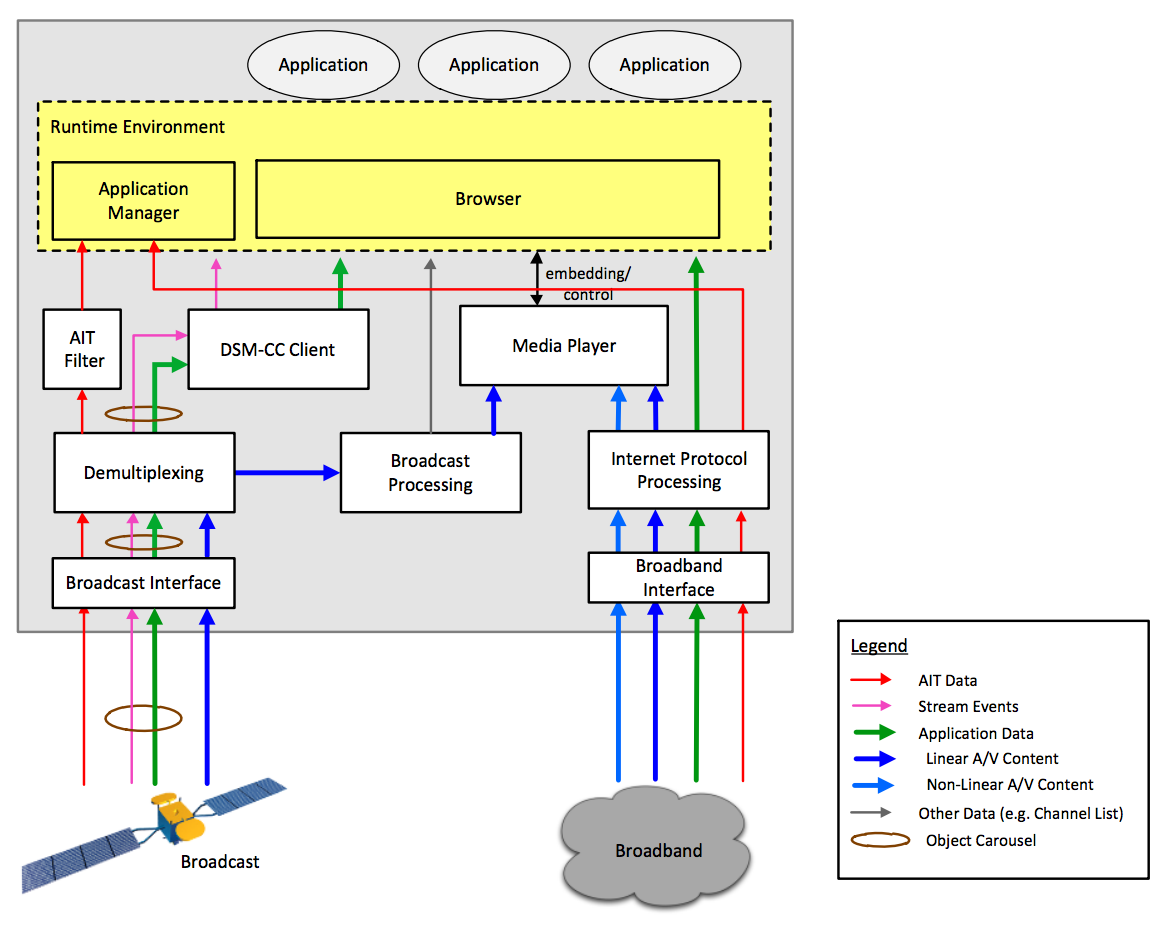
\includegraphics[width=15cm]{app_env.png}\\
  \caption{
    Functional components of a hybrid terminal
  }
  \label{fig:app_env}
\end{figure}

In order to allow the HbbTV app to embed the running broadcast stream within the application the
as a video the Media Player component is required which receives that data after the broadcast
stream was processed. It can also receive A/V content from the broadband source in linear or non
linear form.

As described in section \ref{sec:hbbtv} once the HbbTV application is loaded via broadband stream
it starts either directly by the end-user by pressing a dedicated button on the remote control, in
response to an event stream or by an already running application, e.g. when the user wants to open
an application within the application. With HbbTV version 2 it became also possible to start the
app with a companion screen. However it is often the case that the app is a broadcast related
autostart application which displays a \textit{''Red Button''} notification to inform the user
that an application is available. These are called \textit{''Red Button''} applications. To not
disrupt the video stream they only show something like a small image and leave the rest of the
screen transparent using CSS. This has been agreed in a guideline to not annoy the viewer with
undesired overlays and to allow a uniform experience for the application start. If no action
is taken by the user this indicator disappears again. Since radio services don't have this
indicator, because they don't use the video channel, the full user interface will be displayed.
Some applications like digital teletext apps are not run with autostart enabled. They have
to be specifically triggered by the user without, in this case using the teletext button on
the remote. Triggered one time it starts the digital teletext which is an HbbTV based application.
If triggered twice it closes this app and starts the standard old fashioned teletext. By pushing
the button for the third time it closes also that.

HbbTV apps are not only tied to a specific broadcaster. The so called broadcast-independent
applications \textit{''can be electronic programme guides (EPGs) or “TV editions” of existing
web services such as flickr, YouTube and very many more that may be provided by the big brands
as well as on a regional level or even by individuals.''}\cite{biapps}

\subsection{Development of HbbTV Applications\label{sec:devofhbbtv}}

As mentioned in \ref{sec:hbbtv} HbbTV applications are written in CE-HTML which is an XHTML
based standard to build webpages for consumer electronics like televisions. With the release
of HbbTV version 2 support for HTML5 was added which allows developer to use the latest
web technologies in their apps. Until the majority of devices have support for that apps will
still delivered in the CE-HTML format. Per specification the doctype of the document needs
to be either XHTML 1.0 strict or has to have an HbbTV specific declaration which is

\vspace{1cm}
\begin{listing}[H]
\begin{minted}[mathescape, linenos, numbersep=8pt, gobble=0, framesep=2mm]{html}
<?xml version="1.0" encoding="UTF-8" ?>
<!DOCTYPE html PUBLIC "-//HbbTV//1.1.1//EN"
  "http://www.hbbtv.org/dtd/HbbTV-1.1.1.dtd"
>
<html xmlns="http://www.w3.org/1999/xhtml\">
  <head>
    <meta http-equiv="Content-Type"
          content="application/vnd.hbbtv.xml+xhtml; utf-8"
    />
\end{minted}
\caption{Beginning of an HbbTV document}
\label{lst:doctype}
\end{listing}
\vspace{0.5cm}

Also the document needs to contain an XML decleration at the beginning of the document as well
as a namespace definition in the html tag. This is required so that the device can properly
interpret the document as CE-HTML. In addtition to that the page needs to be served with a
\textit{''application/vnd.hbbtv.xml+xhtml''} content type otherwise the app is going to be
ignored by the television. The browser window has a fixed size of 1280x720 pixel and therefor
fits perfectly in full screen on a 16:9 device. With embedded objects the developer can access
APIs that are defined by the Open IPTV Forum in the HbbTV spec to receive TV capabilities
and configuration as well as access the application manager. It extracts information out of
the AIT packages such as lifecycle of the app or the autostart flag. APIs are available for
configuration and settings, download manager and content download as well as parental access
control and scheduled recordings. However most HbbTV apps these days only need the following
embedded objects:

\vspace{1cm}
\begin{listing}[H]
\begin{minted}[mathescape, linenos, numbersep=8pt, gobble=0, framesep=2mm]{html}
<object type="application/oipfApplicationManager" id="oipfAppMan" />
<object type="application/oipfConfiguration" id="oipfConfig" />
\end{minted}
\caption{Embedded Objects used to access HbbTV APIs}
\label{lst:embeddedObjects}
\end{listing}
\vspace{0.5cm}

Using the DOM node id developers can query the element and access the API. This usally happens
on the \textit{''onLoad''} event that gets triggered onced all DOM elements and JavaScript files
are loaded. The event callback then executes some sort of initialization method that loads the
applications and shows it on the screen.

\vspace{1cm}
\begin{listing}[H]
\begin{minted}[mathescape, linenos, numbersep=8pt, gobble=0, framesep=2mm]{javascript}
var oipf = document.getElementById(appMan);
var app = oipf.getOwnerApplication(document);
app.show();
\end{minted}
\caption{HbbTV App initialization}
\label{lst:loadApp}
\end{listing}
\vspace{0.5cm}

The only input device for HbbTV web apps is the remote control. Within the initialization process
an event listener is registered on the window global object that gets triggered on keydown events.
Depending on the event key code the app executes different actions and allows navigating through
the app.

Since uploading changes to a production server is inefficient and time consuming people have
developed some tool to improve the development environments of HbbTV app developer. There is a
Firefox plugin that emulates an CE-HTML like environment in the browser called FireHbbTV\footnote{\url{https://addons.mozilla.org/en-US/firefox/addon/firehbbtv/}}.
It simulates the TV Remote control using the standard keyboard, displays the safe-area margin as well
as supports most of the HbbTV specific APIs. Another popular tool is the Opera TV Emulator\footnote{\url{http://www.operasoftware.com/products/tv/tv-developer-tools}},
a virtual machine that emulates an Opera SmartTV environment. With that you can have your app being
served on your local machine and easily access it using these tools. However even though these are
helpful tools \textit{''they don't offer the full capacities and facilities that a certified HbbTV
device will provide.''} \cite{hbbtvenv}. Therefor many developers tend to build their apps directly
on the TV with some sort of debug overlay that prints custom debug messages.

\subsection{Available test solutions\label{sec:availabletestsolutions}}

Most of the standard static code analysis tools like JavaScript or CSS linter also apply for HbbTV app
development. These tools ensure that the code can be parsed by the TV device. Specifically for
HbbTV apps the \textit{''Institut für Rundfunktechnik GmbH''} authored a validator\footnote{\url{http://hbbtv-live.irt.de/validator}} that checks
for common pitfalls. It not only warns you if you serve the app with a wrong content-type
it also makes sure that other specifications are met like having the right doctype or required
XML namespace attributes set. However these helper can only detect obvious issues that are relevant
to all HbbTV devices. Problems that only appear on TVs from certain manufactures can not be found
with these kind of tools. It usually requires manual work which ends up being very tedious and
expensive. There are some companies that tried to solve this problem.

A Czech company called Suite.st has developed a system to run e2e tests based on a web GUI on
arbitrary devices either in a remote office or in a local environment. It allows to run these
tests in parallel and provides a comprehensive report about the test result over time. The
GUI allows their user to simply click together one or multiple test scenarios where common
actions are open the app via URL, press a button on the remote and assert that a certain element
contains a certain property. Every aspect of your test can be seperated into sub steps and
reused in other tests. The main idea is that you don't need any coding skills to put together
a test. Figure \ref{fig:suitest} shows how simple the GUI looks like and how tests are being put
together.

\begin{figure}[htb]
  \centering
  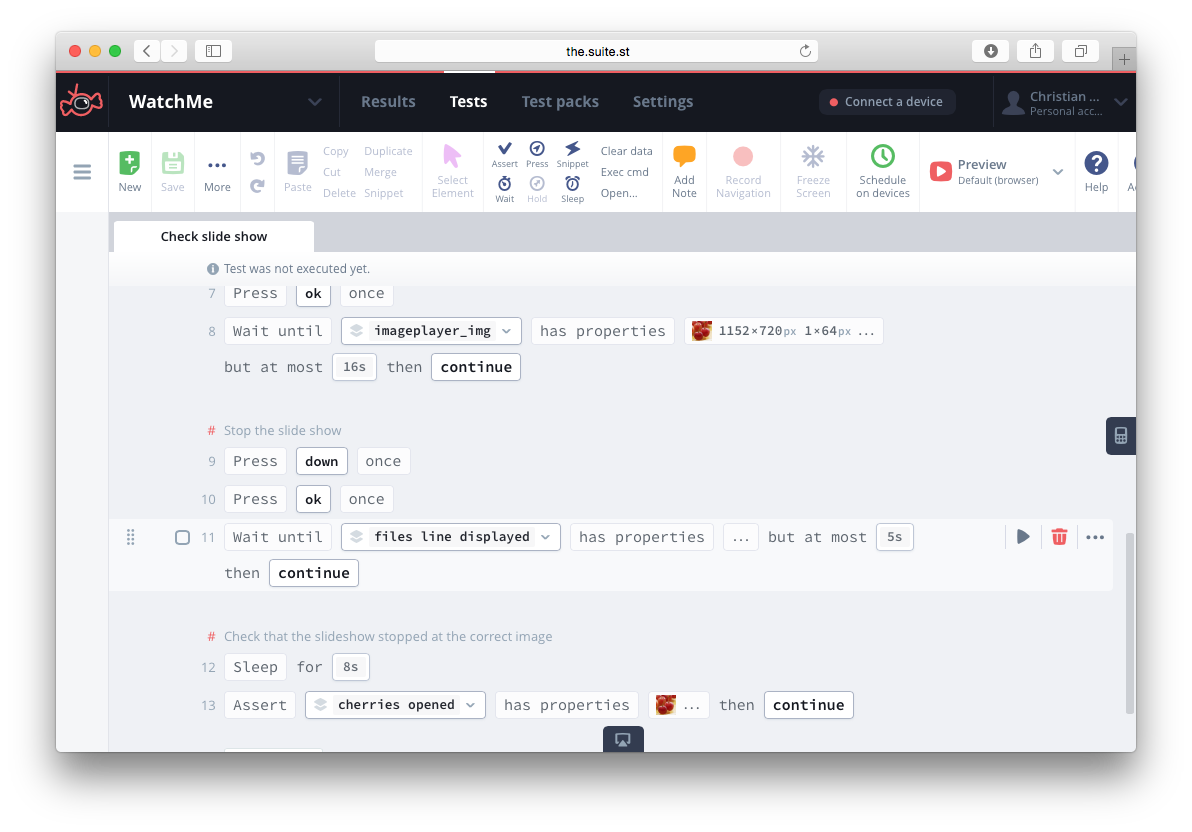
\includegraphics[width=15cm]{suitest.png}\\
  \caption{Suite.st Test Editor GUI}\label{fig:suitest}
\end{figure}

To gain access to the device the company provides a setup box that comes with infraret blasters
in order to simulate remote control events. You can also inject a script into your HbbTV app
to instrument either your browser or TV device to allow Suite.st to run your tests. In case
you don't own a targeted device Suite.st provides a handful of devices from their own datacenter.
It requires a paid plan though which start with 156\euro{} up to 899\euro{}.

Another company providing an e2e test solution for HbbTV apps on Smart TVs is \textit{Eurofins Digital Testing}\footnote{\url{http://www.eurofins-digitaltesting.com/}}.
Next to HbbTV applications they also offer multiple device types such as Set-Top Boxes, standard
web-apps or mobile apps on tablets and phones. Their TestWizard Manager\footnote{\url{http://www.eurofins-digitaltesting.com/testwizard/infrastructure/}}
controls a set of set of TestWizard Robots that contain a different variety of devices depending
on the requirements of the application. Unlike Suite.st the company offers a development tool
called \textit{ScriptStudio} that allows customer to also write automated tests \textit{''without
requirement for extensive knowledge of scripting languages''} \cite{scriptstudio}. Since other
devices types that they offer for mobile and desktop can be tested via test automation scripts
it is also possible to write e2e tests via Selenium and Appium. The company itself is with
22,000 employees way bigger than Suite.st. They have a network of more than 200 laboratories and
offer complete testing solutions not only for HbbTV but also for other key technologies and standards
such as DVB or DASH.

\subsection{Web Platform Tests}

Within the last decade many organizations including the W3C tried to build standards around
technologies that we use everyday. Even though these specifications were adapted by developers
and companies there was still a lack of conformance, quality of implementation, performance
and interoperability. In 2013 the W3C launched \textit{''an unprecedented effort to scale up
its test offering''} \cite{w3ctesting} in which they tried to improve the test infrastructure
and documentation around all web standards that are defined by them. By streamlining the
contribution and reviewing processes they simplified the way how everyone can be involved in
defining and testing a standard. They published their tests and made them accessible for everyone
so that anybody was able to get a clear picture of which web features are supported in whatever
application they are testing. With that every browser vendor was able to make sure that its
browser is working according to the spec. They became the major contibutor for writing and
maintaining these. However the W3C also encouraged every developer to be involved in this
endeavour by starting a movement called \textit{''Test the Web Forward''}\footnote{\url{http://testthewebforward.org/}}.
This was one of major reasons why standards like HTML5 and other technologies that are part
of the HbbTV specification got relieable implemented in many browser and platforms.

The HbbTV specification which was defined within the European Telecommunications Standards
Institute did something similar to ensure that TV manufactures only sell devices that are
complaint to the spec. This is important as \textit{''lean-back consumers have zero patience
meaning any malfunction in the chain will significantly reduce engagement and impact and
may even result in viewers switching to another service''} \cite{hbbtvtesting}. In case of
and update in the standard the association has to make sure that older applications are
interoperable with furthcomming receivers and can coexist with them especially since devices
are not easily updated by the consumer. Therefor they defined a receiver specification and
a device and application conformance that sets certain guidelines and restriction to manufactures
and developers to fulfill the standard and enforce on a common sense. Similar to the W3C a
test suite is provided to manufactures \textit{''to certify their own devices or have their
devices certified by an HbbTV Registered Test Centre.''} \cite{hbbtvtesting}. Once they are
certified they can use the official HbbTV logo for their device products as proof for compliance
to the spec.

\section{Test Automation\label{sec:testautomation}}

There is a lot of different ways on how to test software. Depending on its type and the scope of
the tested functionality there are multiple testing methods that can be applied. From unit testing
that only covers individual software components and code segments to load testing which makes sure
that a specific performance metric is met these methods are used at different stages of the
development lifecycle. With test automation these testing methods can be executed with use of
special software that controls the execution of tests and compares the actual outcome with a
certain predicted outcome. This happens in an automated fashion so that the test itself is mostly
triggered by a certain event (e.g. code changes) in a CI/CD like environment.

From the agile world where coding and testing are one process a concept developed by Mike Cohn
became popular that describes how \textit{''an effectitve test automation strategy calls for
automating tests at three levels: unit, service an UI''} \cite{testautomation}. It explains
that \textit{''unit testing should be the foundation of a solid test automation strategy and as
such represents the largest part of the pyramid''} \cite{unittesting}. On the other side
user interface tests which are placed at the top of the pyramid should be as small as possible
as they are brittle, error prone and time consuming. However they simulate real user scenarios
and ensure that the functionality is working on all levels, from database over the backend
to the user interface. According to Googles philosophie \textit{''focus on the user and all
else will follow''} you could convince someone that writing only e2e tests is a good idea
even though it would object the test automation pyramid. Many developers follow this bad
practice of having to many e2e tests (inverted pyramid or ice cream cone pattern) or a lot
of unit and e2e tests but almost not integration/service level tests (hourglass pattern). A good
rule of thumb here is splitting tests into 70\% unit tests, 20\% integration tests and 10\%
e2e tests. Especially when working as an HbbTV app developer the desire to test apps directly
on multiple TVs is high due to the high fragmentation in the market.

Testing software from end to end is a hard problem to solve. It either requires manual work
which costs a lot of time or engineering effort to automated this process. Over the last
years the tech industry shifted from manual QA to automated testing. Software development
has become more agile with shorter release cycles and feedback loops. Especially due to the
growing popularity of DevOps, development and operations teams are no longer soiled and
engineering work take up the entire application lifecycle, from building the app to test and
deployment. This allows not only to innovate for customers faster and adapt better to changes
in market, it also forces you to increase the frequency and pace of releases in order to
improve the product faster overall. Software these days is \textit{''an integral component
of every part of the business''} \cite{devops}. One fundamental practice in DevOps is
Continuous Integration and Delivery. It improves the software quality by running automated
tests on regular bases after code changes were comitted. Once tests have passed developers
can automatically push their code to production with a high level of confidence that no
regressions were introduced. This can only accomplished with proper tooling. In order to test
software from end to end a framework called Selenium has become the tool of choice for many
developers.

\subsection{Selenium\label{sec:history}}

Selenium is a set of tools and libraries to automated mainly web browsers. It can interact
with them to simulate user actions like click or inputs and assert certain states of web
applications. Those libraries are open source and available in almost any code language and
are used to automate e2e tests. It is supported by all the major browser where each one
provides some sort of automation driver that speaks the Selenium/Webdriver protocol. The
communication is based on HTTP requests between an automation server and the client. Each
test automation is coupled to a session id. Once a sessions is initiated you can communicate
with the automation server via rest API. Such server can be either a Selenium server or directly
a browser automation driver. A Selenium server is some sort of load balancer in order to run
multiple tests on different browser at the same time. It manages all initiated sessions and
reroutes them accordingly. A browser automation server can register itself to such a server
to make itself available for others to use. It allows to speed up your tests by running them
on multiple browser at the same time. You can even run these on different machines or VMs in
your network by using a Selenium-Grid. This allows you to run tests concurrently on different
operating systems and environments. By starting the Selenium server as hub you can connect other
servers on different machines to it. These servers are referred to as nodes. The hub keeps
track on all node configurations and ensures that all requests are load-balanced to them. It
acts as a central access point to all browser in the network.

\begin{figure}[htb]
  \centering
  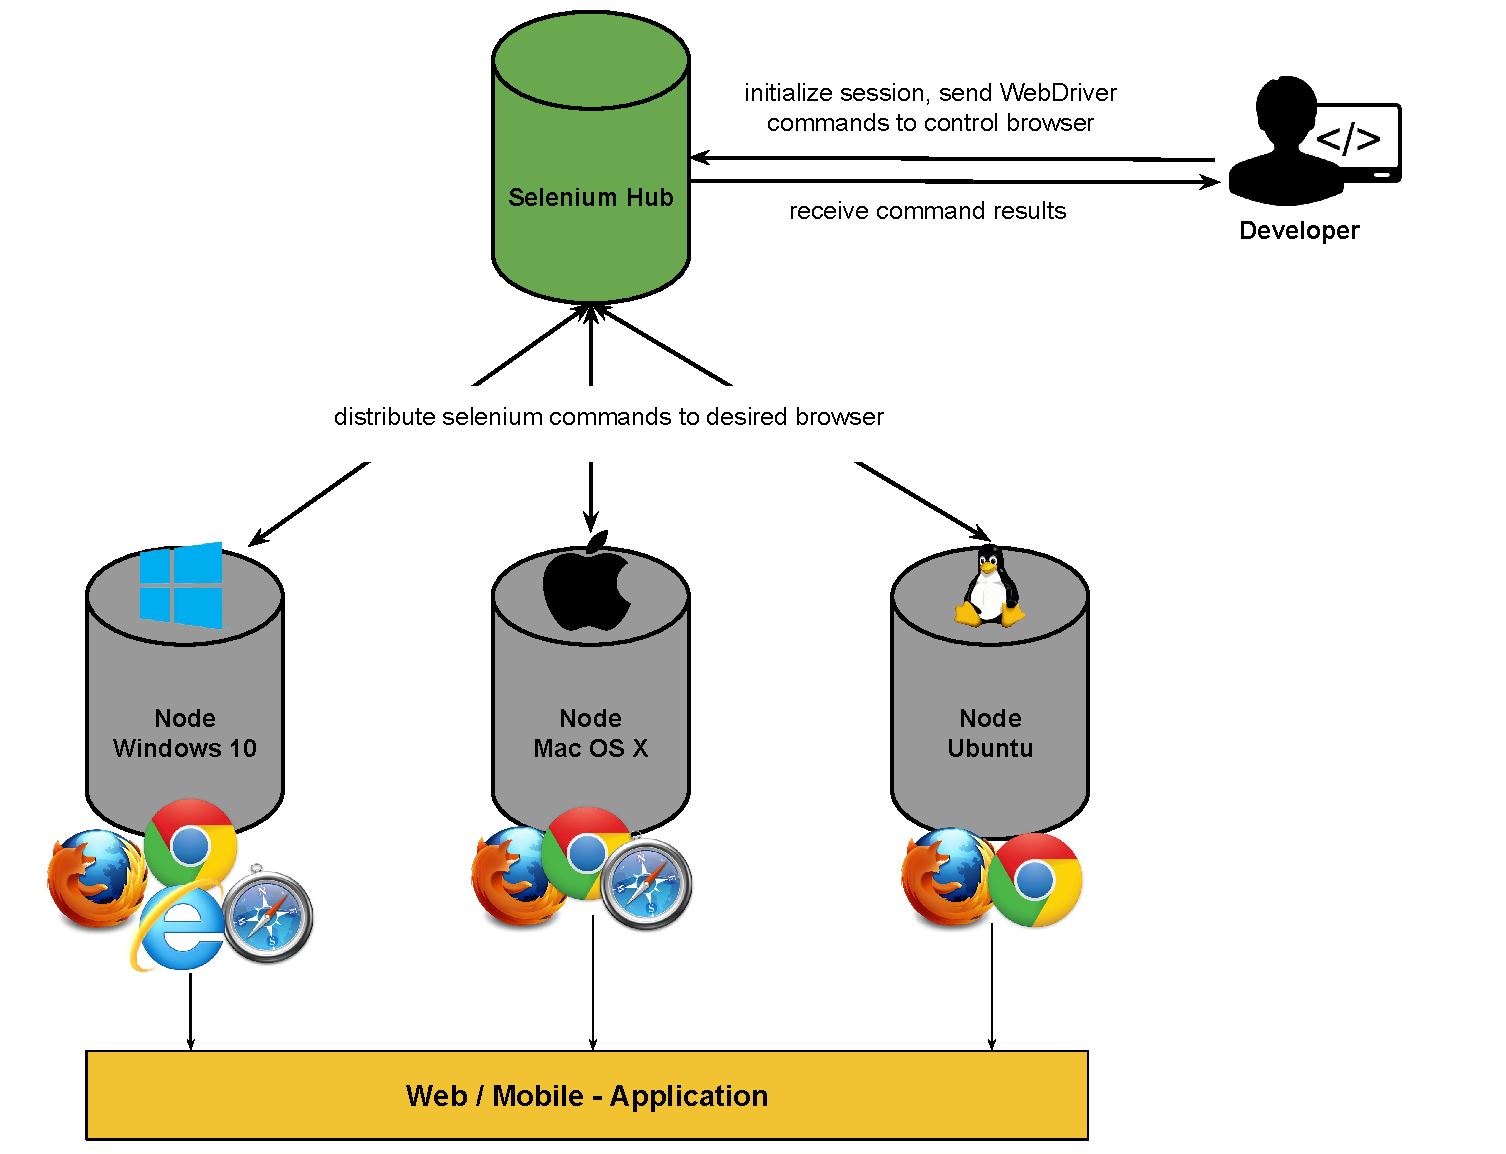
\includegraphics[width=15cm]{selenium.pdf}\\
  \caption{Concept Flow of a Selenium Grid}\label{fig:selenium}
\end{figure}

It is important to point out difference between Selenium and WebDriver here. Selenium was
developed in 2004 by Jason Huggins, an engineer at Thoughtworks\footnote{\url{https://www.thoughtworks.com}}
who tried to build a tool to test web applications that require frequest testing. The tool
was called \textit{JavaScript Test Runner}. It was able to interact with the web page in order
to call certain actions on it. Due to the Same Origin Policy that was introduced by browser
vendors to prevent JavaScript from accessing data of pages that are not within the same domain,
Huggins and his team had to build a proxy server to overcome this. It injected a script to the
webpage to talk to the proxy server and therefor enable the interaction with the webpage. This
proxy server was released to public as Selenium Remote Control and is the first version of
Selenium. In 2007 Simon Stewart who was also working at Thoughtworks build another tool to run
browser tests which he called WebDriver. His tool was not a proxy. It communicated with the
browser directly to use its own engine for automation. In 2011 both tools got merged into one
project that was called Selenium WebDriver (or Selenium 2.0). Over years it became the number
one choice of developers for browser automation so that originators and the community around
the project decided to make the Selenium protocol (also called JsonWireProtocol) a W3C standard.
In 2016 this standard was released by the consortium as candidate recommendation after it was
fully implemented in two major browser (Firefox and IE). It was officially called WebDriver
specification. Even though Selenium and WebDriver are referencing the same project and technology
it still differs in some minor specification details. The Selenium project itself nowadays only
contains the tools that can be used to run tests with WebDriver. Every part that was responsible
to automate the browser became obsolete after all browser vendors stepped up to implement the
automation engine directly into the browser.

\subsection{Appium\label{sec:appium}}

After the success of Selenium and the growing market of mobile devices and applications the
demand for automating mobile phones increased more and more. Even though the big player in
the market (Apple and Android) did provide tooling to create automated tests it still was
time consuming and cumbersome as both platforms forced developers to use their own platform
specific technologies. With that it not only took twice as long to build the app since they had
to be written in Java for Android and Objective-C for iOS respectively, they also had to be
tested with two different frameworks. Appium aims to solve this problem by providing a cross
platform solution for native and hybrid apps. It allows developer to write automated e2e tests
on both platforms using the WebDriver protocol. It extends that protocol to introduce mobile
specific actions like swipe or touch gestures to the developer. Moreover Appium supports hybrid
applications as well which are mobile web apps that are wrapped within a tiny native container
so that you can write one single app and deploy it for both platforms. With that it can also
run a random web page on a browser on the mobile device. Since it leverages the native test
automation frameworks it doesn't matter if you run your test on an emulator or simulator on your
computer or a real device that is setup in a test lab. As the WebDriver protocol is universal
it doesn't require to write tests for Appium in a certain language. Similar to Selenium it is
possible to write tests with any tool that supports the protocol. It also allows to connect
to a Selenium grid to not only have a browser but also a mobile farm available to use for
automated tests.

\section{Chrome Remote Debugging Protocol\label{sec:remotedebuggingprotocol}}

As described in section \ref{fig:selenium} when Selenium merged with WebDriver they started
to communicate with the browser directly in order to interact with the page. As the first
automation driver for Google Chrome was released it used an internal protocol called Chrome
DevTools Protocol to instrument and debug the web page. It is mostly used by the Chrome
DevTools which is a developer tool to inspect the wepage and profile the underlying rendering
engine called Chromium. The protocol is divided into a number of domains where each
\textit{''domain defines a number of commands it supports and events it generates''}
\cite{devtoolsprotocol}. If the user activates a flag\footnote{\url{e.g. in Windows:
chrome.exe --remote-debugging-port=9222}} when starting the browser a TCP server is initiated
and the API can get accessed via a WebSocket connection. This allows to connect to the
protocol via a WebSocket connection and control the browser in any way remotely. The protocol
itself is comprehensive and allows besides receiving information about the state of the page
a lot of debugging and profiling tools. Since it is part of WebKit which is the layout engine
for many browsers - including Chrome (which uses a fork of WebKit called Blink), Safari or
Opera - it allows to drive and debug many browsers. Due to the number of already existing
integrations (including Chrome DevTools) it almost makes it an universal protocol for
automating the browser.

    \chapter{Requirements\label{cha:chapter3}}

The development of HbbTV applications these days is cumbersome and difficult to develop and test.
Even though tools like FireHbbTV\footnote{\url{https://addons.mozilla.org/en-US/firefox/addon/firehbbtv/}}
seems to have found developers interest and attraction the workflow is still not even close to
current industry standards in web development. Tools like Selenium and Appium have prooven that
there is an high demand for developers being able to do develop and test their software in a real
life environment.

With the shift to a more agile software development in the industry it also proofs the demand
to run automated tests in an iterative and quick development cycle. This can only happen
with proper tooling. Software development in browsers or on mobile devices already successful
entered that space of rapid development and quality ensurance using CI/CD. A tool that
tries to bring HbbTV app development to the same point has to build on this strategy. Since
HbbTV apps are not much different to normal webapps in their core technology it would be confusing
and unhelpful if continuous integration and continous delivery would be a different process here.
Therefor the tool has to be based on existing standards around automated testing and development.
It should not only support a seamless integration to already existing tools but also allow
developers to keep their current common practices in building apps similar if not equal to other
areas of web development.

The referred tool will be as outlined in section \ref{sec:scope} and more detailed descriped in
the concept section of this thesis (section \ref{cha:concept}) a piece of software seperated
into two components. Both have individually different requirements. The main goal of the first
component called \textit{Devtools Backend} is to provide developers an integration to the
Chrome Devtools so that they can inspect and debug their HbbTV applications. The other
component called \textit{Appium HbbTV Driver} will based on that component and should enable
to run automated tests based on the WebDriver protocol for arbitrary HbbTV applications on
arbitrary SmartTVs. Both components should be easy to use and integrate into a common and
familar development setup of web engineers.

% Functional requirements may be calculations, technical details, data manipulation and processing
% and other specific functionality that define what a system is supposed to accomplish.
\section{Functional Requirements\label{sec:reqsuba}}

\textbf{Devtools Backend}
- able to integare into standard development tools like Chrome Devtools
- work with arbitrary HbbTV apps
- support any TV Device
- should not break HbbTV pages
- should keep HbbTV app within a black box as good as possible

\textbf{Appium HbbTV Driver}
- transform WebDriver commands into Remote Debugging protocol commands
- has to integrate into existing automated testing tools
  - be used by any Selenium/Appium client
  - support for latets WebDriver specs
  - adapt TV specific attributes (that are not within WebDriver)
  - has to integrate with Selenium Grid to allow multiple TVs

\section{Technical Requirements\label{sec:techreq}}

The following subsection outlines the technical requirements to Component X.

\textbf{Interoperability}
\\
Lorem Ipsum...
\\
\\
\textbf{Scalability}
\\

\section{Social Requirements\label{sec:socreq}}

- e2e tests are hard, so this tool should be easy to use
- similar test tools out there already  it should be better

Component X must compete with Y. Hence, it is required to provide an excellent usability.
This includes ...

    % Chapter 4 is usually termed 'Concept', 'Design' or 'Model'. Here you describe your approach, give a
% high-level description to the architectural structure and to the single components that your solution
% consists of. Use structured images and UML diagrams for explanation. This chapter will have a volume
% of 20-30 percent of your thesis.
%
% This chapter introduces the architectural design of Component X. The component consists of
% subcomponent A, B and C.
%
% In the end of this chapter you should write a specification for your solution, including
% interfaces, protocols and parameters.

\chapter{Concept\label{cha:concept}}

This section will explain in more detail the concepts of each individual component and how they will play together. They individually contribute to the overall goal of implementing a development and test automation platform to build HbbTV applications. The DevTools Backend service will be the base component and will help us to achieve the first part of building a state of the art web-authoring experience. It enables new possibilities for developers to inspect an HbbTV app and understand and debug JavaScript problems within the code. It helps to instrument the application and also to run automated WebDriver tests with the Appium HbbTV Driver. This component acts as translator between the WebDriver protocol and the Remote Debugging Protocol. To do that on a bigger scale we need the Raspberry Pi to deploy that driver to any TV without any manual steps. To manage all these drivers we then use a Selenium Grid and with a proper CI/CD server we can leverage that setup to test and release our HbbTV apps faster and with more confidence.

\section{Components\label{sec:components}}

\subsection{DevTools Backend\label{sec:devtoolsbackend}}

The DevTools Backend is the main component of the overall design. It has to do most of the work and is the only component that directly interacts with the targeted environment: the HbbTV application. Debugging an HbbTV application these days is almost impossible. Even though some TV manufactures provide some interfaces and APIs to connect to the TV they are barely documented and almost different for each TV model. To provide a tool that covers all TVs of all manufactures, it requires a different approach than hooking into a native interface. Until all manufactures recognize the demand for developers to get a better development support this won't change. We already had a similar situation a couple of years ago when the smartphone market started to explode and a lot of people started writing mobile or hybrid apps for Android and iOS. At that time both vendors had almost no support for any debugging tools that would help developers to inspect the page. A tool called \textit{Weinre}\footnote{WEb INspector REmote - \url{http://people.apache.org/~pmuellr/weinre/docs/latest/Home.html}} was developed and found a lot of popularity within the developer community. It enabled to debug arbitrary web pages remotely for the first time, especially on a mobile device such as a phone. It used a unique approach that allowed to do that for all mobile environments (Android, iOS and Hybrid web applications run by PhoneGap/Cordova). After vendors started to support remote debugging natively due to the success of this project it became obsolete and the inventor stopped maintaining it.

This project is the role model for the DevTools Backend component. Similar how it allows to remote debug applications for smartphones, the DevTools Backend will allow it for HbbTV based apps on Smart TVs. The idea is simple. A script that gets executed within a targeted environment connects to a server to exchange information and commands as utility for a 3rd party authoring tool. The concept works independently from the environment and device. As long as the target supports basic web technology like HTML and JavaScript it will run everywhere. This component can not only be used to debug HbbTV apps on Smart TVs but also to inspect any other IoT device like a fridge or a coffee machine as long as their interfaces are based on web technologies\footnote{In fact the screen in the Tesla Model S is build on top of a proprietary web browser and therefor all Tesla apps are build with web technology. Theoretically the DevTools Backend can be used to debug these apps with modern web authoring tools already today.} \footnote{An example application can be found here: \url{http://dash.time4tesla.com/}}.

The component itself consists of two subcomponents. Similar to \textit{Weinre} it has a frontend part that takes care on instrumenting the target environment and a backend part which is a server that initializes and manages the data traffic between target environment and authoring tool. Both subcomponents have logic to handle methods or trigger events according to the Remote Debugging Protocol. As stated in section \ref{sec:remotedebuggingprotocol} the Remote Debugging Protocol is supported by all WebKit browser and has first class support for one of the most used web authoring tools these days: the Chrome DevTools. In addition to that it is actively maintained by a dedicated team at Google and is well documented\footnote{\url{https://chromedevtools.github.io/devtools-protocol/}}. In order to provide as much integration without any additional effort it only makes sense to rely on a well maintained protocol like this.

When it comes to debugging an HbbTV application there will be always three parties involved. The instrumentation logic, the backend and the authoring tool. The instrumentation logic is what actually interacts with the target environment. It executes commands that it receives from the backend and returns desired information. Since the instrumentation script is not much more than any other script on the page it can't support all methods that are defined within the Remote Debugging Protocol. However the JavaScript API is pretty comprehensive and covers the essential requirements of that protocol like returning and modifying the state of certain properties like e.g. DOM nodes. Many things can be emulated which is sufficient for this use case. It is important to ensure that the instrumentation script doesn't affect in any way other scripts or the web application in general from behaving differently. It has to keep its environment as pristine as possible. As a debugging tool it should help developers to find bugs and not create them. Once an instrumentation script was injected into the environment it has to register itself to the backend. Script and backend establish their connection via WebSockets. Since events and methods will be exchanged randomly from both sides it is important to have a full duplex connection type so both ends can communicate with each other in an asynchronous fashion. To identify the target, the instrumentation script has to identify itself with a unique id that can be either the host of the HbbTV app or a randomly chosen string. The backend will register the page based on that id and some other metadata and will manage any connections to it so that arbitrary clients can connect to the page with the backend as proxy. Due to some house keeping work the backend will never directly connect a client to the instrumented page. In fact it will manage the communication with two different WebSocket channels. Not all method requests from clients are directed to the page itself. For example all methods of the Remote Debugging Protocol that relate to network events or page lifecycles are handled by the backend. Figure \ref{fig:command_handling} shows the activity between all parties in more detail.

\begin{figure}[htb]
  \centering
  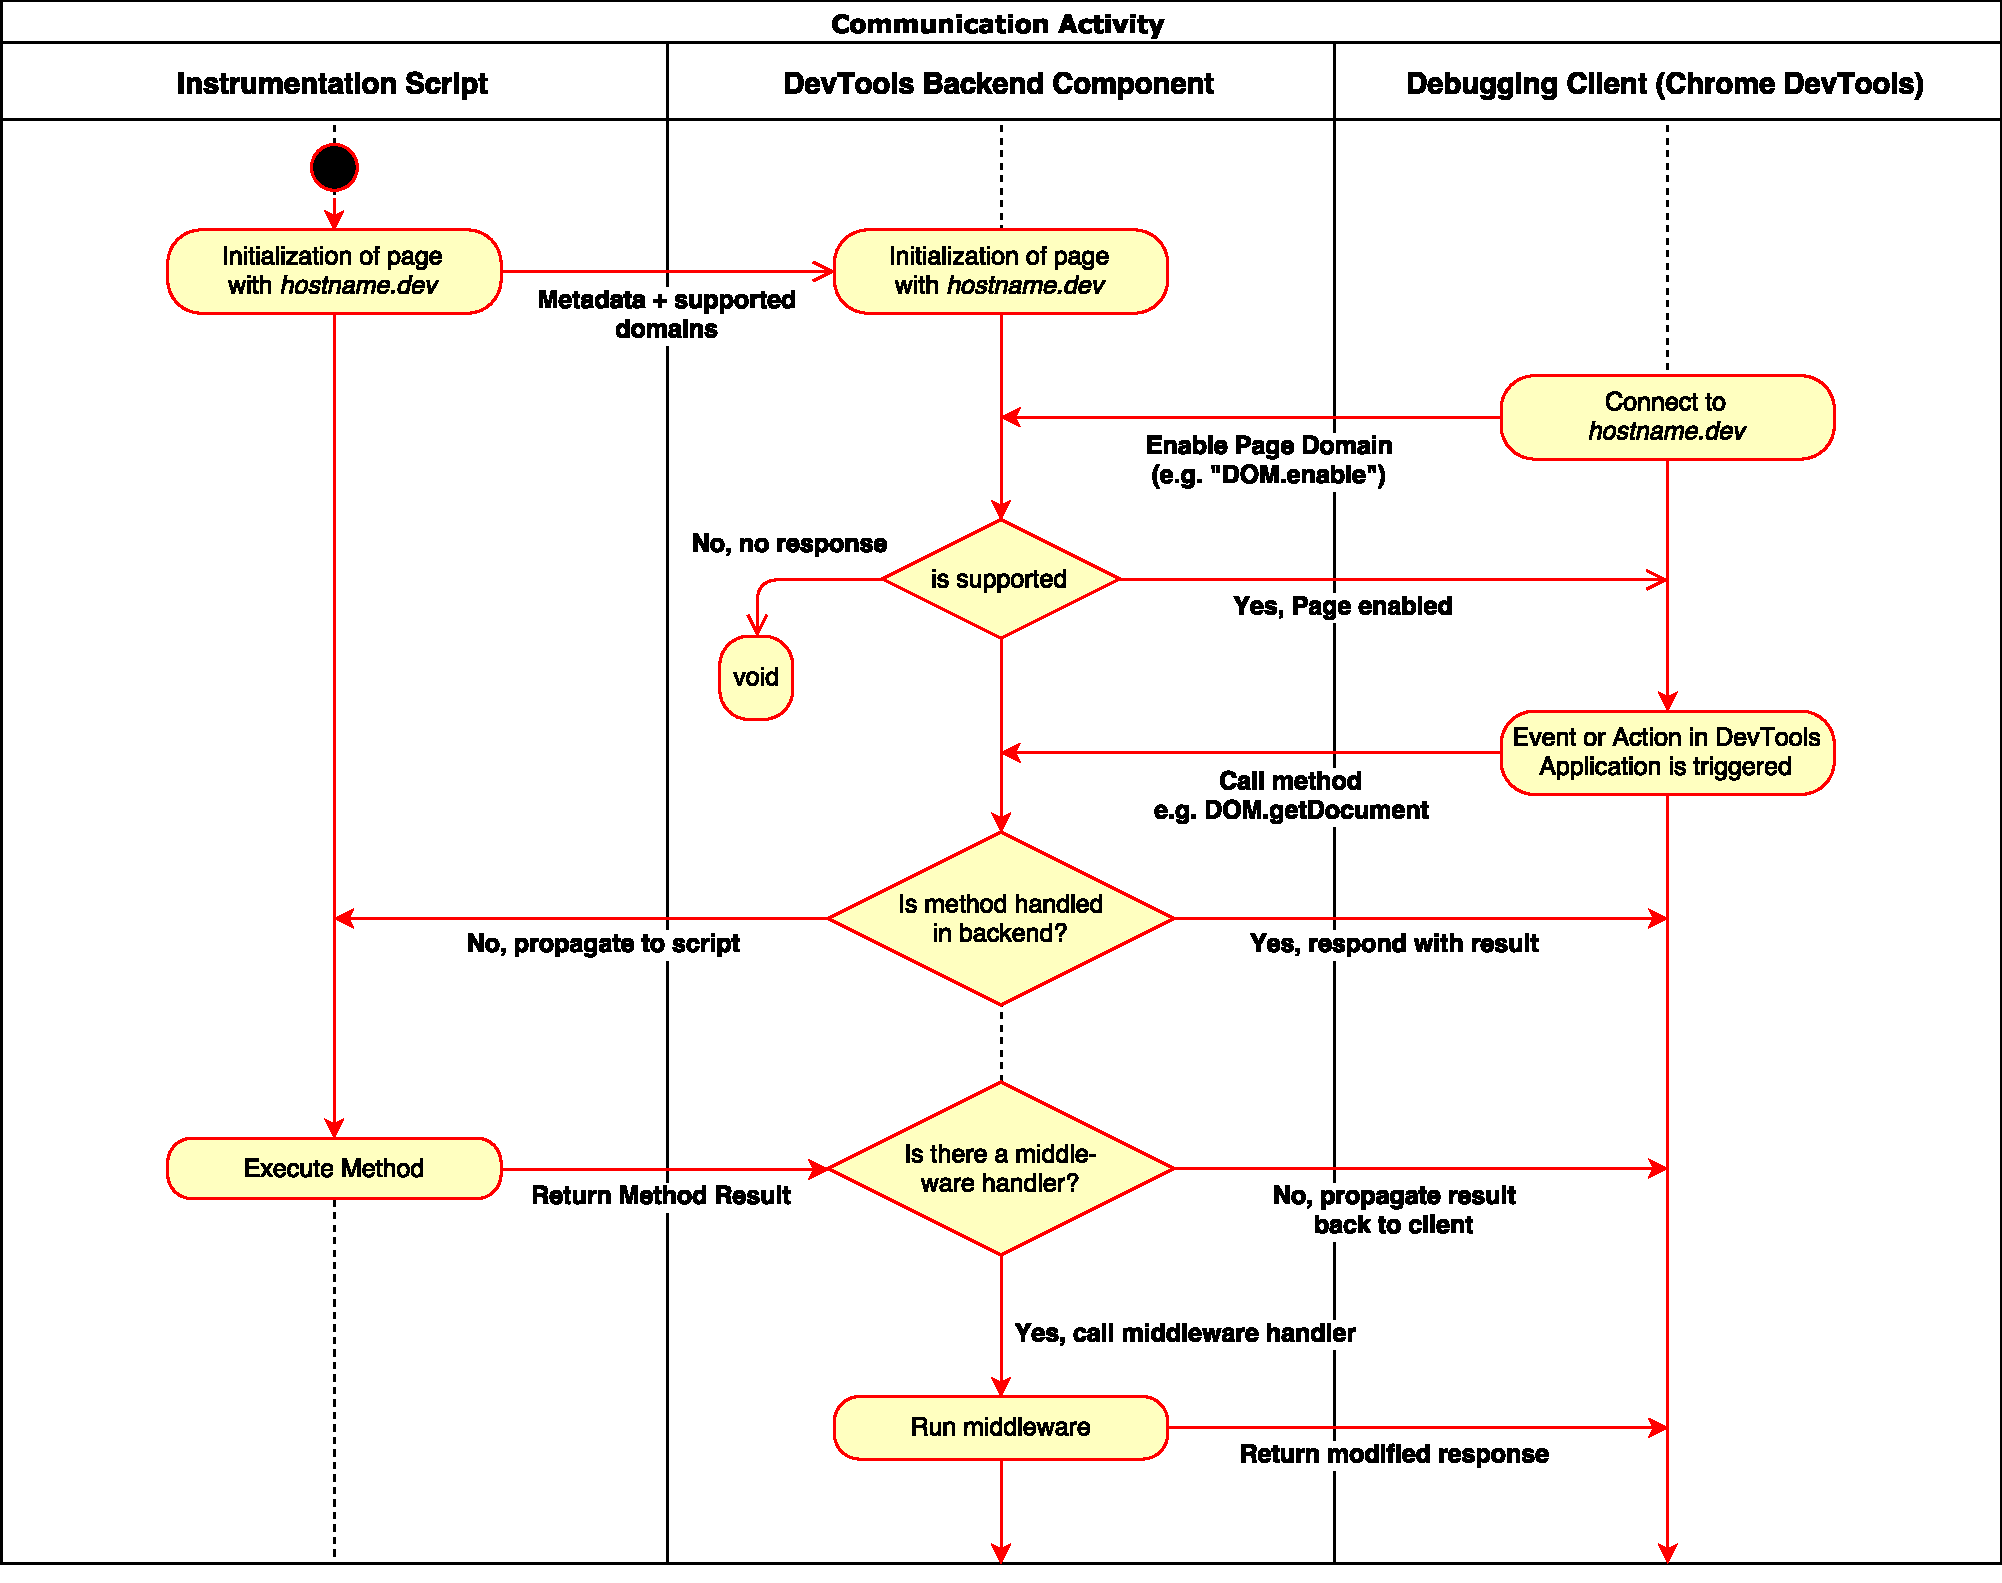
\includegraphics[width=15cm]{command_handling.pdf}\\
  \caption{Communication Activity between Instrumentation Script, Backend and Debugging Client}\label{fig:command_handling}
\end{figure}

In scenarios where a full page load happened the instrumentation script looses the connection with the backend. It manages to reconnect to the target, given that the page unique id is still the same, and makes sure it propagates the right lifecycle events to the connected clients. They won't recognize any connection abruption and instead properly handle the page load on their side. In some cases the response of the instrumentation script needs to be enhanced with data from the backend. This happens when network data is involved which is only stored on the backend side. A middleware handles this situation by enhancing the result object before returning it back to the client.

There are two ways to inject the instrumentation script into the target environment. It can be either placed manually into the page by referencing the script via script tag or the DevTools Backend can be used as a proxy. In this case it captures all http packages on a certain port (usually port 80) and injects the script inline into the page automatically. The proxy registers the page to the backend based on the data it gets from the request. This has the advantage that the application doesn't have to get modified to instrument it. However running the target device (e.g. the Smart TV) through a proxy is not always possible. Therefor the component provides a launcher script that can connect to the backend to register the page before the instrumentation script gets initiated.

Once this happened and a remote debugging client connects to the backend they both exchange JSON payload over the socket channels. The client usually listens to certain domain events (depending on the use case) and fires methods with an id, a method name containing the domain and the request (e.g. \texttt{CSS.getMatchedStylesForNode}) as well as some parameters that get propagated to the method (e.g. a node id). Each domain has to get enabled by the debugging client so that the communication can be reduced to the minimum. If the client would enable all domains it would overflow the socket channels. This keeps the data amount manageable. The backend only propagates messages to the instrumentation script if the containing method was enabled by the client beforehand. Even though all methods and events of the protocol are documented in a comprehensive way\footnote{see \url{https://chromedevtools.github.io/devtools-protocol/}} the order of events and methods that have to get triggered on both sides is unknown. The only way to find out when certain events has to get thrown is by debugging the debugging tool. Since the Chrome DevTools is just a normal web-application it is possible to debug it using the Chrome DevTools itself. Within the \textit{Timeline} tab it is possible to inspect the WebSocket connection to the browser in real time. This allows to reverse engineer the protocol and emulate a similar behavior like in the browser.

\subsection{Appium HbbTV Driver\label{sec:appiumhbbtvdriver}}

Based on the DevTools Backend component the Appium HbbTV Driver is now able to run its automated tests without having to take care about how to automate WebDriver commands on the TV. Since the DevTools Backend is applicable to all HbbTV supported devices the driver can therefor be utilized on arbitrary TVs or SetUp boxes supporting that format. It uses the already existing framework utilities provided by Appium to support all common functionalities that an automation driver requires. Appium already provides a variety of drivers that are mainly focused on mobile automation. However its vision is to create more drivers that support new devices and platforms. HbbTV is the perfect fit for that. With Appiums Basedriver module\footnote{\url{https://github.com/appium/appium-base-driver}} it provides not only a template to build the driver but also comes with all required features to run it on bigger scale e.g. within a Selenium Grid out of the box. An overview about all involved components is shown in figure \ref{fig:hbbtv-driver-components}.

\vspace{1cm}
\begin{figure}[htb]
  \centering
  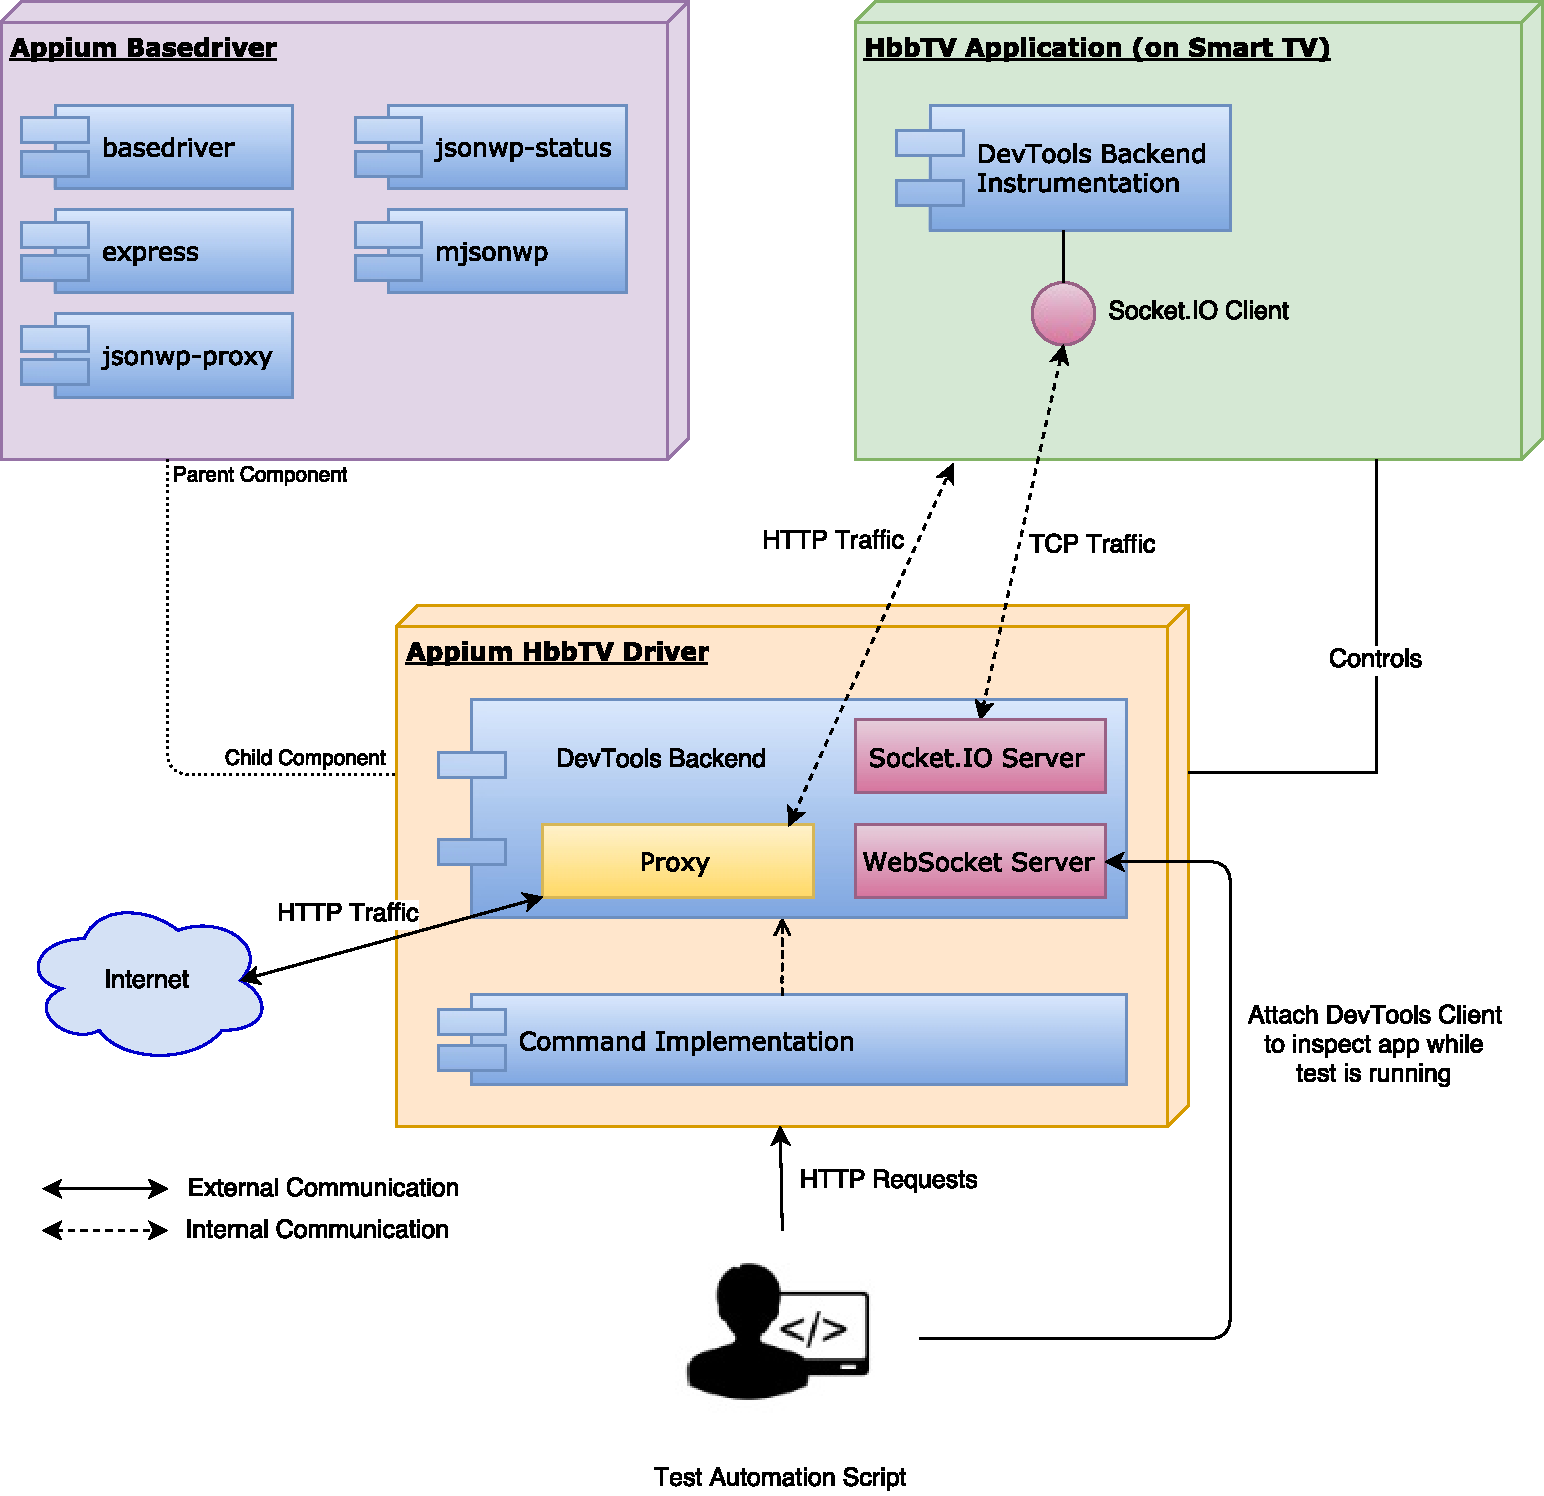
\includegraphics[width=15cm]{hbbtv-driver-components.pdf}\\
  \caption{Appium HbbTV Driver components}\label{fig:hbbtv-driver-components}
\end{figure}
\vspace{0.5cm}

Thanks to Appiums Basedriver a lot of important functionality can be inherited. It builds the foundation of the actual driver. It takes care of session management and capability definition/validation (\textit{''basedriver''}), provides predefined WebDriver routings (\textit{''mjsonwp''}) which are served by a preconfigured HTTP server component (\textit{''express''}). With that it manages incoming HTTP requests and handles their responses by applying the correct response codes (\textit{''jsonwp-status''}). That also allows additional features like proxying these requests (\textit{''jsonwp-proxy''}). Since it is using the Appium framework on one side and the DevTools Backend on the other the only task of this driver is to translate the WebDriver commands into the Remote Debugging Protocol. WebDriver commands are send as normal HTTP requests. The driver acts as a restful HTTP server and can receive these request. Depending on the endpoint it triggers a different action on the target device. Every automated test starts by initating a WebDriver session. Figure 4.2 demonstrates this process in detail.

\vspace{1cm}
\begin{figure}[htb]
  \centering
  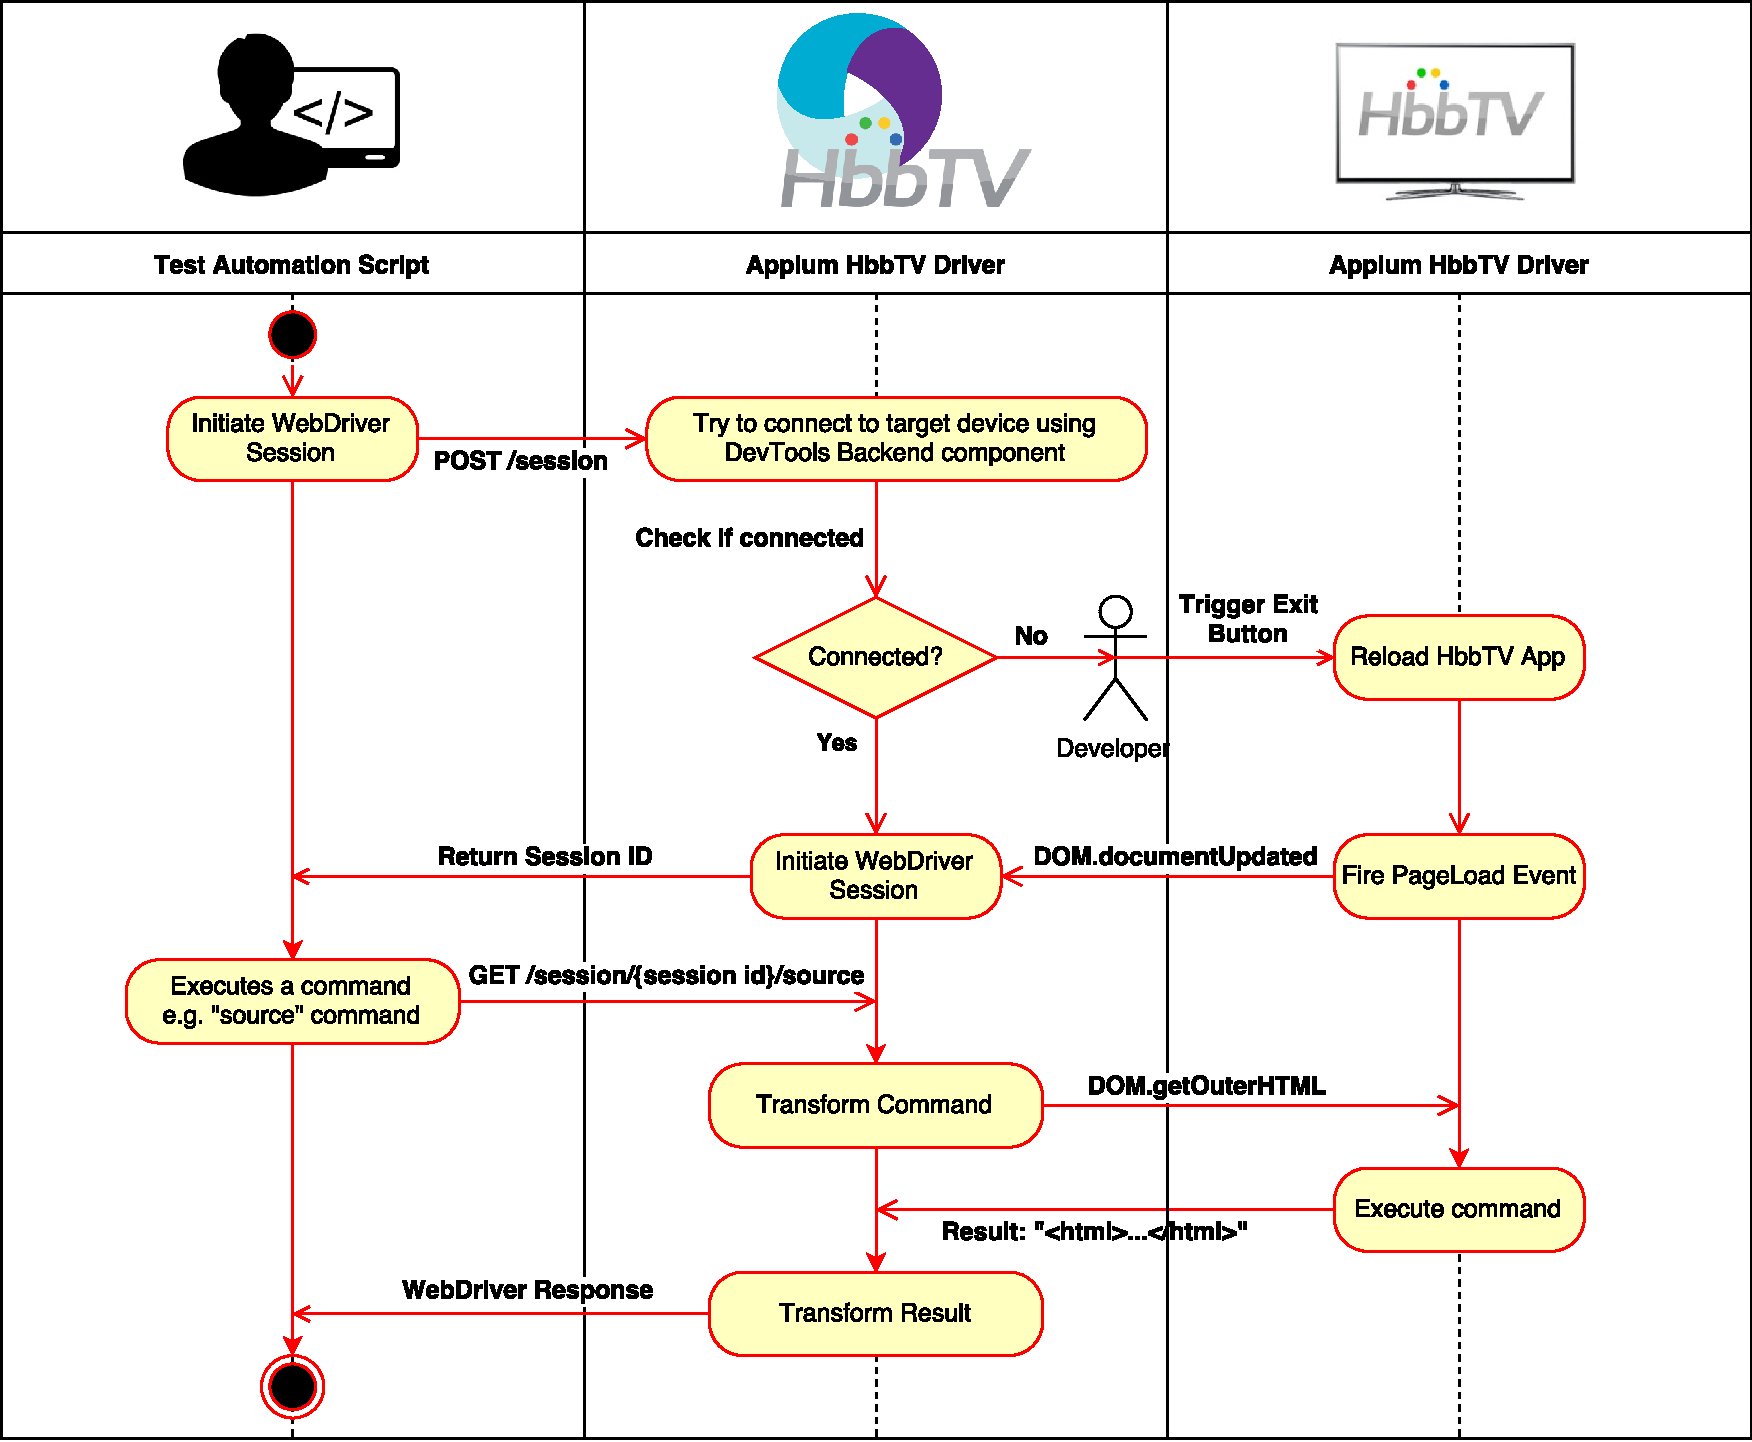
\includegraphics[width=15cm]{appium-driver-diagram.pdf}\\
  \caption{Creating A WebDriver Session}\label{fig:appium-driver-diagram}
\end{figure}
\vspace{0.5cm}

A session can only be successful initiated if the DevTools Backend component is able to successfully connect to the target device. In case the TV is turned off or never got instrumented by the DevTools Backend it requires one manual step to finish the initiation process. By pressing the Exit button on the remote the HbbTV app gets reloaded and the DevTools Backend can inject the script if used as a proxy. If the instrumentation script is injected manually the test script can connect to it by providing the page ID within its capabilities. Once a connection to the target device was established the initial session request can be resolved. The response includes a session ID next to other information of the assigned device. The session ID is important as it is part of almost all WebDriver endpoints to identify the user and execute all commands on the right device.

Depending on the test framework of the developer the session ID gets automatically stored within the test context. The developer can now run any WebDriver commands. After the driver has received a new command it transforms it into a Chrome DevTools Protocol method and forwards it to the DevTools Backend component. Since the Dev- Tools Backend is using an asynchronous socket connection the driver has to wait until either the result of the method was returned or a certain event was triggered in order to resolve the WebDriver HTTP request. Certain commands can trigger a page load in the target environment that will break the connection between the DevTools Backend component and the instrumentation script. In these cases the driver has to wait until a reconnection happened in order to resolve the request, otherwise the test script would not be able to send the next command. If the connection can't be re-establised a timeout will be hit and causes to return with an error.

\subsection{Raspberry Pi\label{sec:pi}}

To ensure that such connection loss never happens a man in the middle component between network and Smart TV can be used. A peripheral like a Raspberry Pi\footnote{https://www.raspberrypi.org/} is an ideal utility to manage a TVs network traffic and instrument any HbbTV app on the fly. A Raspberry Pi is a \textit{''fully customizable and programmable small computer board''}\cite{raspberrypi} with a size of a credit card. It has a 1.2GHz 64-bit quad-core ARMv8 processor with 1 GB RAM, 4 USB and 1 Ethernet port. It is known as the mainstay in the world of makers and electronics but also as an educational device that brings people the joy of electronics and computer programming. With 38\euro{} it is super cheap and yet powerful. People who are familiar with Linux have no problems to start building tools and applications with it. With a prebuild Raspbian operating system the provisioning of a TV to test HbbTV apps can be reduced to a simple plug\&play step.

The idea is that all network traffic of the Smart TV runs through the Raspberry Pi. Running the DevTools Backend component it acts as a Proxy between TV and network. This has the advantage that every HbbTV app will be instrumented on the fly. There is no need to manually inject an instrumentation script. The DevTools Backend proxy modifies every HTTP package that has an HbbTV mime type before it sends it back to the TV. In addition to that it tracks all application assets so that the developer can inspect all files that have been downloaded by the HbbTV app including information like request and response headers. This setup allows to not only do that with own applications but also with any HbbTV app of any broadcaster that can be received by the Smart TV. Having said that, it allows to monitor all communications between HbbTV app and server and helps to understand how certain applications track your behavior while using the app.

In order to put this together, it requires an additional ethernet cable as well as an USB to Ethernet adapter. The Raspberry Pi has to maintain two network interfaces. One is for the data transfer between TV and Pi and the other for the one between Pi and network. Therefor you could theoretically also use the Wifi module to connect to your network instead of using the USB adapter. With the correct network setup it should connect automatically. Once it is connected to the power supply the operating system boots up and starts the Appium HbbTV Driver. To identify the Raspberry Pi we change the hostname settings to be the model name of the TV it is connected to. After the Pi has established a connection between TV and our network we can immediately address this host as our automation server and run tests on it.

\vspace{1cm}
\begin{figure}[htb]
  \centering
  
\includegraphics[width=15cm]{pisetup.pdf}\\
  \caption{Setup of SmartTV with Raspberry Pi}\label{fig:pisetup}
\end{figure}
\vspace{0.5cm}

To seperate the network traffic we have to run both interfaces on different subnets. This can be customized depending on the given network. Most local networks will have an IP range of \texttt{192.168.1.1/24} which is why this setup would make the most sense as default. However once a proper network is found it is possible to copy the images to other Raspberry Pis. This will allow us to provision an already existing TV lab in a simple way and deploy our components to run automated WebDriver tests using the Appium HbbTV Driver and DevTools Backend.

\section{Selenium Grid\label{sec:grid}}

To run our automated tests on multiple TVs with different HbbTV support at the same time we need a Selenium Grid to orchastrate the WebDriver requests. The Appium HbbTV Driver component allows us to register to such a grid using an internal settings page that the user can open in the browser. The only information that is required is the IP address of the Selenium Grid server. That server has to be accessible in the network where the TV and the Raspberry Pi are located in. The driver will send a request to the Selenium Grid server containing the capabilities of the TV. In order to receive those from the device it is important that the DevTools Backend is able to connect at least once with an HbbTV app to identify the TV by looking on its user agent. It always constains the supported HbbTV version as well as the name of the manufacturer and device model. If the registration to the grid server was successful it will automatically ping the Raspberry Pi every once in a while to check its connectivity and status.

\vspace{1cm}
\begin{figure}[htb]
  \centering
  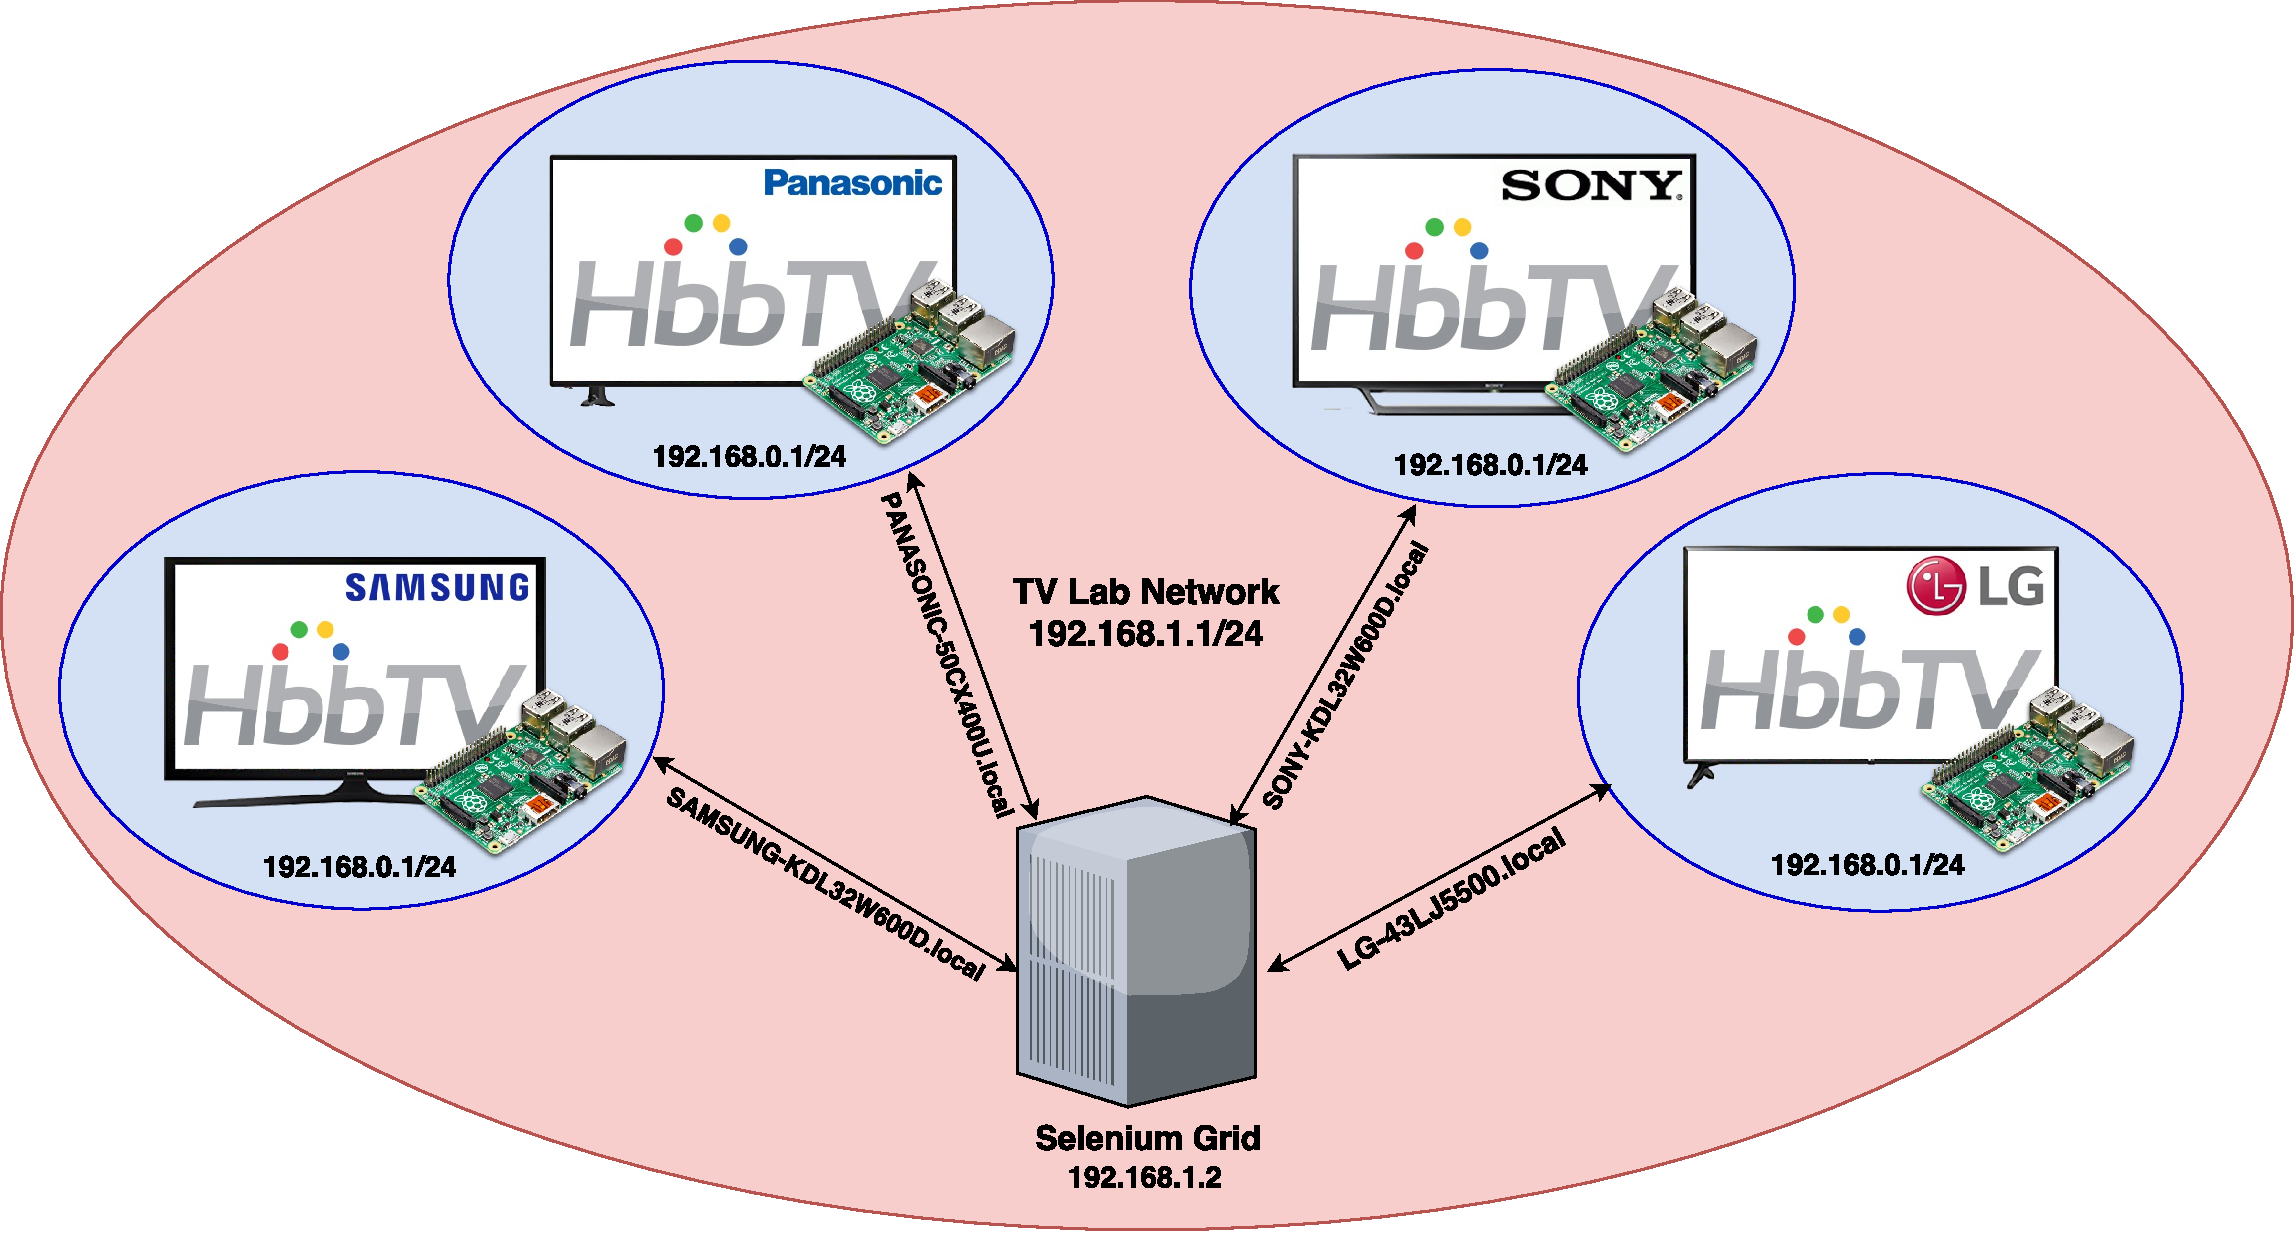
\includegraphics[width=15cm]{network.pdf}\\
  \caption{Network Setup of TV Lab with Raspberry Pi}\label{fig:network}
\end{figure}
\vspace{0.5cm}

The Selenium Grid will be the access point for all developers to run their automated tests on. It manages its capabilities and only creates a session if the desired device is available and not used by someone else. If a device is blocked due to another test it will queue up the request and waits until it becomes available again. Each Smart TV is registered with the supported HbbTV version, the name of the manufacture and its model name. Each test can therefor specify on what kind of device it should be running. The Selenium Grid tries to find the best suiteable device if available. If for example the developer wants to run a test on a Smart TV with supported HbbTV 1.5 the grid server randomly selects a Smart TV that runs that HbbTV version. The same goes for other capabilities. All data about registered Smart TVs and their availability can also be consumed as JSON blob using the Rest API of the grid server. This allows creating custom dashboards that are more aligned to the TV theme. Instead of just model names it could display the TV model as image with the manufacture logo.

\section{Continuos Integration and Delivery\label{sec:cicd}}

The last step to have a fully automated continuous integration and delivery pipeline is to setup an automation server that runs our tests as soon as any code changes were introduced to the project. There are multiple ways to setup such pipeline. CI/CD became a major part in the software delivery process over the last years so that many tools have been developed since then. One of the most popular open source solutions is Jenkins\footnote{\url{https://jenkins.io/}}. It is \textit{''deployed at large scale in many organizations''}\cite{jenkins} and \textit{''has no licensing costs''}\cite{jenkins}. In combination with a source control tool like Git\footnote{\url{https://git-scm.com/}} we can trigger our automated tests regularly so that defects are detected at early stage before it is deployed to production. Depending on the project and its requirements you can deploy different strategies on how code gets tested and pushed to a production environment. This can be fully automated so that no human interaction is necessary anymore.

% ToDo: explain CI/CD process of HbbTV app

    % Chapter 5 describes the implementation part of your work. Don't explain every code detail but emphasize
% important aspects of your implementation. This chapter will have a volume of 15-20 percent of your thesis.
%
% This chapter describes the implementation of component X. Three systems were chosen as
% reference implementations: a desktop version for Windows and Linux PCs, a Windows Mobile
% version for Pocket PCs and a mobile version based on Android.

\chapter{Implementation\label{cha:implementation}}

Since we are working in a web environment it only made sense to build all software components with a
popular web technology too: JavaScript. Both the DevTools Backend and Appium HbbTV Driver components
are written in NodeJS using a Babel\footnote{\url{https://babeljs.io/}} compiler to use the latest
EcmaScript features today. They both use Eslint\footnote{\url{http://eslint.org/}} for static code
analysis and have a Dockerfile so they can get seamlessly deployed on any system that has Docker\footnote{\url{https://www.docker.com/}}
installed.

\section{DevTools Backend\label{sec:implDevtoolsBackend}}

The DevTools Backend has a simple NodeJS project structur with a \textit{package.json} that contains
a handful of CLI commands to operate and build the project. It is stored on the Fraunhofer GitLab
server and can be cloned with git if permissions are granted. Once it was cloned you can simply install
the dependencies and build it using the NPM commands. The project requires to run a NodeJS version
of v7.4.0 as defined in \textit{.nvmrc}.

\vspace{1cm}
\begin{listing}[H]
\begin{minted}[mathescape, linenos, numbersep=8pt, gobble=0, framesep=2mm]{shell}
# clone project
$ git clone git@gitlab.fokus.fraunhofer.de:christian.bromann/devtools-backend
# install dependencies
$ cd devtools-backend
$ npm install
# build project
$ npm run build
# run server
$ npm run start
\end{minted}
\caption{Setup DevTools Backend component locally}
\label{lst:setupdevtools}
\end{listing}
\vspace{0.5cm}

With Docker this procedure is simplified down to these commands:

\vspace{1cm}
\begin{listing}[H]
\begin{minted}[mathescape, linenos, numbersep=8pt, gobble=0, framesep=2mm]{shell}
# clone project
$ git clone git@gitlab.fokus.fraunhofer.de:christian.bromann/devtools-backend
# install dependencies
$ cd devtools-backend
$ npm run docker:build
# run container
$ docker run -p 9222:9222 devtools-backend
\end{minted}
\caption{Setup DevTools Backend component with Docker}
\label{lst:setupdevtools}
\end{listing}
\vspace{0.5cm}

The build process not only compiles all server side files down to ES5 using Babel, it also compiles
all frontend related files (the instrumentation code) to one JavaScript file which gets injected
into the HbbTV app. This has the advantage that the structure and the way these files are written
don't differ from each other. Thanks to WebPack\footnote{\url{https://webpack.js.org/}} all frontend
files are bundled together so that they can get executed in the browser. This makes it super easy
to structure and share code on server and frontend side. The main server is build on top of Express\footnote{\url{https://expressjs.com/}},
a minimal and flexible web framework to build web applications in NodeJS. It allows to define API
endpoints and provides useful utility features to work with Cookies and caching. All application code
can be found within the \textit{lib} directory. Next to the main server and proxy logic most of the
code is split up in backend and frontend. The backend part is responsible to route all WebSocket
communication between the remote debugging client (e.g. the DevTools application) and the frontend
automation code that gets executed on the Smart TV. It also tracks all network traffic that comes
through the proxy and returns the data to the client if desired. All backend related information
like registered pages, resource content or metadata are being held there to save the request to the
frontend. For simplicity reasons this data is held in memory.

As \textit{''page''} we define a debugging target that can be either an HbbTV app on a SmartTV or
any other web page where the instrumentation code is injected and connected to the backend. The
server can be used to debug multiple pages at the same time. Each page has an unique identifier
that allows to connect a client on the desired page. The communication between the debugging target
and the server gets initiated via Socket.io\footnote{\url{https://socket.io/}}. Socket.io is a
sophisticated NodeJS module that enables real-time bidirectional event-based communication between
server and client. It is not only super fast and efficient it also works relieable on many web
platforms. Especially on Smart TVs where not all devices have support for WebSockets, Socket.io
ensures that a connection can be established by using fallback strategies like XHR polling. From
the server to the debugging client a standard WebSocket server architecture was chosen since
there are no such fallback requirements to be fulfilled. In addition to that a Socket.io server
can only connect to clients that are using Socket.io as well which is undesired because it should
be accessible by arbitrary clients. Everytime the proxy injects an instrumentation script or the
launcher registers itself to the backend a new page instance is created and two new Socket channels
are opened.

\begin{listing}[H]
\begin{minted}[mathescape, linenos, numbersep=8pt, gobble=0, framesep=2mm]{js}
export default class Page extends EventEmitter {
    constructor (io, uuid, hostname, url, title, description, metadata) {
        super()
        // ...

        this.io = io.of(`/page/${this.uuid}`)
        this.io.on('connection', ::this.connect)

        this.wss = new WebSocket.Server({
            perMessageDeflate: false,
            noServer: true
        })
    }
    // ...
}
\end{minted}
\caption{Socket Channels initiated in Page class}
\label{lst:socketServer}
\end{listing}

It is worth mentioning that the backend doesn't create a WebSocket server every time a page instance
gets initiated. It instead attaches itself to the Express server and creates a fake server instance
(see \textit{''noServer: true''} in listing \ref{lst:socketServer}). When a client asks for a WebSocket connection
an \textit{''upgrade''} event is emitted when the opening handshake takes place. It \textit{''upgrades
the connection from HTTP to the WebSocket protocol''}\cite{socket}.

\begin{listing}[H]
\begin{minted}[mathescape, linenos, numbersep=8pt, gobble=0, framesep=2mm]{js}
// lib/index.js
export default class DevtoolsBackend {
    constructor (host = DEFAULT_HOST, port = DEFAULT_PORT) {
        this.app = express()
        this.server = this.app.listen(port)
        this.server.on('upgrade', ::this.backend.upgradeWssSocket)
        // ...
    }
    //...
}
\end{minted}
\caption{Server Initiation with ExpressJS}
\label{lst:socketUpgrade}
\end{listing}

The backend module keeps a list of all registered pages and can upgrade the connection properly if
the event was fired by the server. Depending on the unique page id (uuid) the backend connects the
debugging client to the desired page and enables the communication between client and instrumentation
code.

\begin{listing}[H]
\begin{minted}[mathescape, linenos, numbersep=8pt, gobble=0, framesep=2mm]{js}
// lib/backend/index.js
upgradeWssSocket (req, socket, head) {
    const pathname = url.parse(req.url).pathname
    for (const page of this.pages) {
        if (pathname === `/devtools/page/${page.uuid}`) {
            return page.wss.handleUpgrade(
              req, socket, head, ::page.connectWebSocket
            )
        }
    }
    socket.destroy()
}
\end{minted}
\caption{Multiple Socket Channels Registered on one Server}
\label{lst:socket}
\end{listing}

Once the connection was established the debugging client can send commands and receive events from
the instrumentation code. In most cases the backend only propagates these messages from Socket.io
to the WebSocket connection and vice versa.

\subsection{Instrumentation Script}

The frontend part of the DevTools Backend component is the instrumentation script. It gets executed
in the target environment, e.g. the HbbTV browser on the Smart TV. It connects to the backend via
Socket.io and is used to propagate page events to the debugging client as well as execute commands
to transform elments or get information about the page state. The instrumentation script should be
placed at the top of the \texttt{<head>} block to ensure that it gets executed before everything
else. This is important because it has to capture as much events as possible. In case the HbbTV app
fails to load due to a JavaScript error it only can propagate that error to the debugging client if
it has registered an error handler before the HbbTV code was executed. It also overwrites certain API
like the console object to intercept messages and events. All methods for a certain Chrome DevTools
Protocol domain are stored in one file. Listing \ref{lst:navigate} shows an example of an implemented
method\footnote{\url{https://chromedevtools.github.io/devtools-protocol/tot/Page/\#method-navigate}}
for the page domain. As mentioned above it is written using the latest EcmaScript language features
like the destructuring assignment syntax\footnote{\url{https://developer.mozilla.org/en/docs/Web/JavaScript/Reference/Operators/Destructuring_assignment}}
or the export statement\footnote{\url{https://developer.mozilla.org/en/docs/web/javascript/reference/statements/export}}.
Even though these features aren't supported in current browsers (and especially not in proprietary
HbbTV browsers of old TV models) they can still be used since the code gets compiled down to a legacy
JavaScript version. This ensures that the code is fully compatible on the target device. However this
doesn't replace missing JavaScript APIs. Therefor any APIs that have not been defined within the
EcmaScript 3 specification, which is the supported version for HbbTV 1.0, is either avoided or used
in a way that it fails silently if not available.

\begin{listing}[H]
\begin{minted}[mathescape, linenos, numbersep=8pt, gobble=0, framesep=2mm]{js}
/**
 * Navigates current page to the given URL.
 *
 * @param  {String} url  URL to navigate the page to.
 */
export function navigate ({ url }) {
    if (typeof url !== 'string') {
        return
    }
    window.location.assign(url)
    return {}
}
\end{minted}
\caption{"navigate" Method of Page Domain}
\label{lst:navigate}
\end{listing}

All domain logic is then imported into a single module to export it as central API. This pattern is called
\textit{''Barrel''} and has its origin from the TypeScript world. \textit{''A barrel is a way to rollup
exports from several modules into a single convenient module. The barrel itself is a module file that
re-exports selected exports of other modules''}\cite{barrel}.

\begin{listing}[H]
\begin{minted}[mathescape, linenos, numbersep=8pt, gobble=0, framesep=2mm]{js}
import * as CSS from './css'
import * as DOM from './dom'
import * as Debugger from './debugger'
import * as Input from './input'
import * as Network from './network'
import * as Overlay from './overlay'
import * as Page from './page'
import * as Runtime from './runtime'
import * as Target from './target'
import * as Webdriver from './webdriver'
export default {
    CSS, DOM, Debugger, Input, Network, Overlay,
    Page, Runtime, Target, Webdriver
}
\end{minted}
\caption{Barrel Module Containing All Domain Logic}
\label{lst:barrel}
\end{listing}

This allows us to import one file containing an interface to access the whole domain logic. With only a
couple of lines we can then register an listener to the Socket.io channel for each domain and execute
a method based on the message parameters.

\begin{listing}[H]
\begin{minted}[mathescape, linenos, numbersep=8pt, gobble=0, framesep=2mm]{js}
import domains from './domains'
for (let [name, domain] of Object.entries(domains)) {
    this.domains[name] = domain
    this.socket.on(name, (args) => this.dispatchEvent(domain, args))
}
\end{minted}
\caption{Register Listeners to Socket Connection}
\label{lst:barrel}
\end{listing}

The \textit{dispatchEvent} method checks if the action that is defined within the arguments is implemented
and executes it if so. It then either returns the result of the function call back to the backend and
debugging client or does nothing if no result was returned. This approach allows us to enhance the domain
logic without having to register new listeners to the socket connection.

To reference DOM nodes back and forth between instrumentation script and debugging client every node on
the page is getting referenced with a node id. As soon as the instrumentation script gets initiated and
the DOM tree is rendered it runs through the whole tree and sets an internal flag (\texttt{\_nodeId}) on
every node. In addition to that it saves a reference to that node internally so it can find it based
on the node id at all times. If a client fetches the document using \texttt{DOM.getDocument}\footnote{\url{https://chromedevtools.github.io/devtools-protocol/tot/DOM/\#method-getDocument}}
the instrumentation script returns instead of the actual node object a representation of it based on
the Node\footnote{see lib/frontend/models/Node.js} class. This representation contains the assigned node
id which allows the client to interact (e.g. change attributes or the content) with that node. In addition
to that every instance registers a mutation observer\footnote{\url{https://dom.spec.whatwg.org/\#mutation-observers}}
on itself. This allows to listen to DOM and attributes changes on DOM nodes and helps debugging clients
to update DOM tree representations in their applications (e.g. Chrome DevTools Elements panel). Other composite
objects like promises, generators or maps are handled similarly. With the PropertyObject\footnote{see lib/frontend/models/PropertyObject.js}
class the instrumentation script converts each object into a different representation of itself to allow
data exchange over the HTTP protocol. Instead of the actual object it returns an object id that is stored
in an ObjectStore\footnote{see lib/frontend/models/ObjectStore.js} on the page. Since these objects can't
be serialized they remain there and can be referenced using the object id. Similar to how DOM nodes are
stored every object in the object store is held in memory. Since every object is passed by reference this
won't have any affect on the performance of the page.

\subsection{Launcher\label{sec:launcher}}

The Launcher script is what's used to manually inject the instrumentation logic on arbitrary platforms
without setting up a proxy. It contains next to the Socket.io client library an initialization part and
the actual instrumentation script. The initialization part is important as the script needs to register
itself as a page to the DevTools Backend component. If a proxy is used this happens usually on the server
side. To inject the launcher a script tag has to be placed at the top of the \texttt{<head>} block so
that it gets executed first. The actual code can be received from the DevTools Backend server.

\vspace{0.3cm}
\begin{listing}[H]
\begin{minted}[mathescape, linenos, numbersep=8pt, gobble=0, framesep=2mm]{html}
<html>
<head>
    <title>My Target Page</title>
    <script src="http://<devtools-backend>:9222/scripts/launcher.js"
            data-origin="debugger">
    </script>
    <!-- ... -->
\end{minted}
\caption{Inject Launcher Script}
\label{lst:launcher}
\end{listing}

Once the script is downloaded by the browser it sends an XHR request to the server with some page metadata
(e.g. uuid, url, title, user agent, etc) asking to register this page to the backend. After that it
initates the instrumentation scripts and starts the communication to the backend via Socket.io. The uuid
can be defined manually by adding a \texttt{data-uuid} attribute to the script tag. If this attribute
can't be found it uses the hostname as unique id. The \texttt{data-origin} attribute is used to hide this
DOM node from the debugging client. If a client requests DOM nodes from the instrumentation script these
node will be ignored so that they don't show up in any DOM representation as they actually are not part
of the web application.

\subsection{Proxy\label{sec:proxy}}

To automate the script injection the DevTools Backend component provides a proxy that modifies the content
of certain HTTP packages. It injects the Socket.io client library and the instrumentation script inline so
that it can establish a socket connection with the backend even before the document has fully loaded.
Since all network traffic will go through the proxy it is able to track all packages that have been
requested by the app. With that information we can provide a full network report for each page load
including timeline information and data on when the first package was loaded and when loading was finished.
Since you can inspect every network package it allows you to see how certain HbbTV applications load data
from the backend as well as how it tracks your behavior on the page.

Since we only want to modify packages that contain HTML code and pass on the other packages, e.g. images
or scripts, we have to make sure that we filter every request depending on its type. This can be done in
multiple ways. Just by extracting the file ending you can already identify most of the packages by its
type. Additional some requests have an \texttt{Accept} header that contains the expected mime type that
is about to be returned by the server. However these information do not fully ensure that the file that
is being requested should be modified or not. Given the fact that modifying a wrong file can break the
whole app we need to have a better way to detect file types. Therefor the proxy has another middleware
registered that makes an \texttt{OPTIONS}\footnote{\url{https://developer.mozilla.org/en-US/docs/Web/HTTP/Methods/OPTIONS}}
request to actually decide whether to pass it forward or to load its content in order to inject the
instrumentation script. The HTTP options method can be used to not only detect available HTTP methods
it also returns the content type of the requested resource. Since the response doesn't contain any body
payload it is really lightweight.

\begin{listing}[H]
\begin{minted}[mathescape, linenos, numbersep=8pt, gobble=0, framesep=2mm]{js}
class Proxy {
    // ...
    proxyFilter (req, proxyRes, next) {
        req.target = getFullUrl(req)
        request.head(req.target).then((headers) => {
            /**
             * only proxy resource if content type is an HbbTV application
             * Note: to act as normal proxy (for other apps than hbbtv) it
             * should also allow normal html content-type
             */
            const contentType = headers['content-type']
            if (contentType && (contentType.match(/hbbtv/g) ||
                contentType.match(/text\/html;/g))
            ) {
                // pass forward to proxy
                return next()
            }
            // ...
            // if not HbbTV application pipe request directly into response
            const requestCall = request(opts)
            return requestCall.pipe(proxyRes)
        }, (err) => /* ... */)
    }
    // ...
}
\end{minted}
\caption{Filter Proxy Request based on Response Content Type}
\label{lst:proxyFilter}
\end{listing}

By calling the \texttt{next()} method we pass on the request to the next middleware which actually handles
script injection. This happens only if the content type contains HbbTV or text/html though. All other
requests are getting logged and directly piped to the response. This only works because the request and
response objects are read/writeable streams.

The proxy not only ensures that the target page gets instrumented it also allows custom modifications to the
browser behavior. It is often the case that you want to demo a certain HbbTV application without having to
setup a broadcast stream that sends an AIT package with the correct address to that app. The DevTools Backend
component provides for that scenario a setup page\footnote{Available at \url{http://<ip-of-raspberrypi>:9222/settings}}
that allows to set up an autostart application. When the Smart TV then asks for an HbbTV app it automatically
redirects the request to the given URL. For the sake of simplicity the autostart url is stored on the filesystem
in a json file and can be access by a helper function.

\begin{listing}[H]
\begin{minted}[mathescape, linenos, numbersep=8pt, gobble=0, framesep=2mm]{js}
/**
 * check autoload settings
 */
const { autoload, whitelist } = readConfig().data
const cues = typeof whitelist === 'string'
    ? whitelist.split(',').map((f) => f.trim())
    : []

if (autoload && !cues.find(cue => req.get('host').indexOf(cue) > -1)) {
    this.log.info(`Autoload URL found, redirecting to ${autoload}`)
    return proxyRes.redirect(307, autoload)
}
\end{minted}
\caption{Redirect option to demo arbitrary HbbTV applications}
\label{lst:hbbtvRedirect}
\end{listing}

As shown in Listing \ref{lst:hbbtvRedirect} the redirect only takes place when a comma seperated list
of keywords is not part of the actual request host. Given that a lot of HbbTV applications contain subpages
and sub applications the developer has to define some keywords that have to be whitelisted. Otherwise
you will always enter the given autoload page when trying to access a subpage.

\section{Appium HbbTV Driver\label{sec:driver}}

Similar to the DevTools Backend component the Appium HbbTV Driver is a Node.JS project that is similar
structured as the DevTools Backend component. The setup as described in Listing \ref{lst:setupdevtools}
is identical. The driver itself doesn't contain a lot of code. Most of the logic is hidden within its
dependencies. As described in section \ref{sec:appiumhbbtvdriver} the Appium HbbTV Driver is using the
DevTools Backend component to run its automation. It runs on a Raspberry Pi so that it uses the proxy
feature of that component to inject the script on any HbbTV app automatically. In this case it will
automatically connect to the page that was modified by the proxy. However you can also run your Selenium
tests on any arbitrary web page that was instrumented by the DevTools Backend instrumentation script.
By having a \texttt{pageId} defined there that matches to the uuid of a registered page in the backend
it can establish a connection to that page to send the DevTools protocol commands. In case the Smart
TV has no connection to the DevTools Backend the developer has to manually restart the app so the proxy
can instrument the HbbTV application. If this doesn't happen the WebDriver session fails.

Once a connection was established the HbbTV driver connects to the WebSocket server of the page (e.g.
the target HbbTV application). Similar to the Chrome DevTools application it will receive a lot of
app information that are propagated from the DevTools Backend component. With that it is able to send
commands to the actual HbbTV page on the Smart TV as well as receive page data. At this point the
WebDriver session could be established successfully and the developer can start to run his first automated
commands. The command handling itself depends on whether or not the request triggers a page load or not.
If it does the driver has to ensure that the DevTools Backend component was able to successfully reconnect
to the page. This only happens if we are able to receive certain events from the component.

\begin{listing}[H]
\begin{minted}[mathescape, linenos, numbersep=8pt, gobble=0, framesep=2mm]{js}
commands.setUrl = async function (url) {
    this.request('Page.navigate', { url }, false)
    await waitForEvent(this.emitter, 'DOM.documentUpdated', TIMEOUT)

    /**
     * implicit pause for page to render
     */
    await new Promise((resolve) => setTimeout(resolve, 500))
}
\end{minted}
\caption{Implementation example of the setUrl WebDriver command}
\label{lst:setUrl}
\end{listing}

The example in listing \ref{lst:setUrl} shows how a WebDriver command\footnote{As defined in the protocol
\url{https://www.w3.org/TR/webdriver/\#go}} is translated to a Chrome DevTools Protocol command\footnote{See
\url{https://chromedevtools.github.io/devtools-protocol/tot/Page/\#method-navigate}} and send to the DevTools
Backend component using an internal helper method called "\texttt{request}". From there it gets propagated
to the actual HbbTV app where the instrumentation script handles the action (e.g. navigate to a page given
by the url in the payload). The third parameter of that function indicates how the driver has to behave after
the command is triggered. A truthy value would make the driver wait for the exact response. This is used
mainly for commands that actually return a value (like a CSS property\footnote{when calling the getCssProperty
command \url{https://www.w3.org/TR/webdriver/\#get-element-css-value}}). In this case however continuing after
the command would be problematic since the page is about to open a new HbbTV application. By passing in a falsy
value it therefor indicates that the command handles the waiting by itself and we expect no response for that
command whatsoever. By calling \texttt{waitForEvent} in the next line we now wait until a custom event is
propagated by the application. In this case we wait for the \texttt{DOM.documentUpdated} event which is triggered
\textit{''when [the] Document has been totally updated [and] Node ids are no longer valid''}\cite{devtoolsprotocolDOM}.
The command resolves once this event was received. At the end of the command we implicitely wait for a half of
a second in order to give the browser time to render the page. Smart TVs tend to be slow in many situations and
the HbbTV browser especially is not always quick in rendering the app. This small timeout stabilizes the
execution flow and prevents the driver from running into arbitrary race conditions.

\subsection{Driver Architecture\label{sec:implDriver}}

Thanks to Appiums ecosystem building a driver is fairly simple. The basic architecture is provided by Appium itself.
The device automation is the only part that has to be implemented and differs between all drivers. When the driver
gets initiated it imports two important modules from the \texttt{appium-base-driver} project which is the main
dependency of the driver. It requires a \texttt{server} module which is an custom express server that handles
all WebDriver requests according to the protocol. This module provides a function that is responsible for registering
all WebDriver endpoints as defined in the protocol. The \texttt{routeConfiguringFunction} method which is also
imported from the \texttt{appium-base-driver} then simply maps\footnote{The mapping is defined in the appium-base-driver
project as well: \url{https://github.com/appium/appium-base-driver/blob/master/lib/mjsonwp/routes.js}} all endpoints
to a certain instance function defined in the Appium HbbTV Driver. With that all requests to e.g. "\texttt{/wd/hub/session}"
to initialize a WebDriver session are automatically mapped to a function called \texttt{createSession} which then
intializies the automation as described in the previous section. The base server not only maps the endpoints to
certain functions it also checks if the payload is correct and valid according to the protocol.

In addition to the protocol endpoints the Appium HbbTV Driver also registers additional views\footnote{see settings
view at \url{http://<ip-of-raspberrypi>:4723/settings}} for the developer to e.g. register the driver to a
Selenium Hub via a simple form. As described in section \ref{sec:history} a Selenium Hub is a central server that
collects multiple driver in order to have a single access point to all automation server. This allows us to register
many Appium HbbTV Driver connected to different Smart TVs to a central point and access all TVs at the same time
through it. It simplifies adding more Smart TVs to a sophisticated TV infrastructure. In order to register a driver
manually to a remote hub the Appium HbbTV Driver also has a custom view\footnote{Available at
\url{http://<ip-of-raspberrypi>:4723/nodeconfig.json}} to receive the node config that is required to register to the
hub. Based on the capabilities defined in that config and in the payload of the WebDriver request the Hub will select
the driver registered with that config.

\subsection{Selenium Grid Setup and Scaling\label{sec:setupscaling}}

The described implementation allows to seamlessly setup and scale a Selenium Grid with multiple TVs from different
manufactures. All you need is a:

\begin{itemize}
  \item Smart TV connected to a HbbTV Play Out
  \item Raspberry Pi, including:
    \begin{itemize}
      \item 4GB SD card provisioned with a predefined image
      \item USB to Ethernet adapter
      \item Ethernet cable
    \end{itemize}
  \item Virtual Machine or another Raspberry Pi running a Selenium Hub
  \item Router that is connected to the internet and all TVs in a single network
\end{itemize}

The Ethernet port of the Smart TV has to be wired with the USB to Ethernet adapter of the Raspberry Pi that belongs
to the TV. The embedded Ethernet port of the Raspberry is then connected to the router. The image on the Pi is
preconfigured so it starts all components automatically. It runs a DHCP server that should assign an IP address to the
SmartTV after booting\footnote{If this is not the case the Raspberry Pi has to be rebooted}. The Pi itself will then
get an IP address assigned by the router. The TV should be then connected to the internet via the Raspberry Pi. The
last manual step is to open a broadcast stream with a HbbTV signal so that the proxy on the Pi can instrument the page.
From that point we can control the HbbTV browser via any WebDriver client. It makes sense to set the hostname of the Pi
to the name of the TV model it is assigned to in order to easier access the right device. You can change the hostname by accessing
the Pi via SSH and open the internal configuration menu\footnote{via "\$ sudo raspi-config"}. If you access the DevTools
Backend component on the Pi via opening a browser at e.g. \url{http://ue46f8090sl.local:9222} you should then see the
list of inspectable pages which at that point should be the HbbTV app you just opened. Note that the DevTools Backend
component is per default registered on port 9222 (standard remote debugging port) and the Appium HbbTV Driver on port
4723 (standard Appium port). Another static server is registered on port 8080 and gives you a list of logs that are
captured from both components.

The image for the Raspberry Pi is preconfigured and has all necessary components installed. You can download it under
the following Owncloud link: \url{https://tubcloud.tu-berlin.de/s/DU6R40CoHvHgVk3}. Using tools like Etcher\footnote{\url{https://etcher.io/}}
you can flash it on a 4GB SD card. As mentioned above make sure to SSH into the PI to configure the hostname. The
default hostname is \texttt{appium-hbbtv-driver} so you can log into the Pi via "\texttt{\$ ssh pi@appium-hbbtv-driver.local}".
The password is the default Raspberry Pi password ("\texttt{raspberry}").

Once you have connected the Pi as described to the Smart TV you can start running automated WebDriver tests on them.
There are hundreds of WebDriver client libraries publicly available\footnote{A curated list of can be found at
\url{https://github.com/christian-bromann/awesome-selenium\#tools}}. If you want to run your test on a specific TV
you can just point the client to the corresponding Raspberry Pi in the network. Using a popular WebDriver client in
JavaScript called WebdriverIO\footnote{\url{http://webdriver.io}} a simple automation script would look like:

\begin{listing}[H]
\begin{minted}[mathescape, linenos, numbersep=8pt, gobble=0, framesep=2mm]{js}
import WebdriverIO from 'webdriverio'

const browser = WebdriverIO.remote({
    host: 'ue46f8090sl.local', // or IP of grid server
    port: 4723, // or 4444 if grid server
    desiredCapabilities: {}
})

browser
    .init()
    .url('http://itv.ard.de/ardstart/index.html')
    /**
     * execute JS on the target device returning the user agent
     */
    .execute(() => navigator.userAgent)
    /**
     * outputs: "HbbTV/1.1.1 (;Samsung;SmartTV2013;T-FXPDEUC-1102.2;;) WebKit"
     */
    .then((result) => console.log(result.value))
    .end()
\end{minted}
\caption{Simple automation script with WebdriverIO to print out the user agent}
\label{lst:wdioExample}
\end{listing}

As shown in the example you don't need to define any capabilities since the automation driver is accessed directly.
Based on that you can build more sophisticated test suites for any kind of HbbTV applications. An example of such
test suite can be found in the demo directory in the Appium HbbTV Driver repository\footnote{\url{https://gitlab.fokus.fraunhofer.de/christian.bromann/appium-hbbtv-driver/tree/master/demo}}

% \section{Setup Evaluation\label{sec:setupevaluation}}
%
% - Raspberry vs injected
% - advantages vs disadvantages
% - when to use what
%
% \section{TestBed Setup\label{sec:testbed}}
%
% - How we integrated it in Fame TestBed
% - Show off grid
% - Demonstrate use cases
% - How to run a Selenium test
%
% \subsection{Deployment\label{sec:deployment}}
%
% - How to add another TV
% - How are they connected
%
% \subsection{Continues Delivery of HbbTV Apps\label{sec:cicdhbbtvapps}}
%
% - How to setup an HbbTV project with CI/CD running tests on TestBed
%
% \subsection{Reporting of Test results\label{sec:reporting}}
%
% - How to leverage universal usage thanks to common protocols
% - demonstrate Allure reporting

    \chapter{Evaluation\label{cha:chapter6}}

In this chapter the implementation of Component X is evaluated. An example instance was
created for every service. The following chapter validates the component implemented in
the previous chapter against the requirements.\\
\\
Put some screenshots in this section! Map the requirements with your proposed solution.
Compare it with related work. Why is your solution better than a concurrent approach from
another organization?

\section{Business model\label{sec:businessmodel}}

- What do they try to solve
- Patent

\section{Features and Offerings\label{sec:features}}

- Explain provided features

\section{Solution Evaluation\label{sec:usab}}

- Compare solutions
- For which group of people is which solution the better choice

\section{Comparison of writing automated tests for web/mobile vs TV\label{sec:diffInWritingTests}}

- Compare Inpute devices
- JS and environement feature set

    \chapter{Conclusion\label{cha:chapter7}}

% Chapter 7 summarizes the thesis, describes the problems that occurred and gives an outlook about future
% work. Should have about 4-6 pages.
%
% The final chapter summarizes the thesis. The first subsection outlines the main ideas
% behind Component X and recapitulates the work steps. Issues that remained unsolved are
% then described. Finally the potential of the proposed solution and future work is
% surveyed in an outlook.

More and more digital devices are getting connected to the internet and run applications that are build with web
technologies. The HbbTV protocol was the foundation of bringing the web on the big screen. This fairly new standard
now encounters the same issues of debuggability and testability as other device and software markets before, e.g.
mobile application development. Til today there is no solution that really addresses these issues. As the HbbTV
standard evolves and the device fragmentation increases the demand for qualitative tools for qualtity assurance
rises too. This thesis solves these issues by connecting established technologies and protocols together to create
a testing and debugging solution that can be integrated in modern software development pipelines.

\section{Summary\label{sec:summary}}

% Explain what you did during the last 6 month on 1 or 2 pages!

The work on this thesis started with an in depth research phase on the HbbTV standard and current testing technologies.
Unfortunately there were no existing solutions found at this point. Some companies like BBC provided some ressources
of their own homegrown solutions\footnote{See BBC Hive Open Source Test Tools (\url{http://bbc.github.io/hive-ci/})}
that are suited for their requirements. However the goal of this work was to find way to make testing and debugging
of arbitrary HbbTV applications accessible to everyone. Therefor it has to be non oppinionated and should not prescribe
a certain way of how to do things. To evaluate the technical opportunities one of the first steps was to discover
the accessibility of a modern Smart TV. Using tools like WireShark a variety of interfaces could be discovered that
allowed mobile applications to e.g. remote control the TV and enable second screen technology. These interfaces also
gave insights on the device capabilities as well as their underlaying software. Given that there were multiple
manufactures with different Smart TV platforms that even have different interfaces based on their models this approach
of controlling a TV device turned out to not be very promising.

Another interesting view point were virtual machines that emulated an HbbTV environment on your operating system.
With the Opera TV Developer tools\footnote{\url{http://www.operasoftware.com/products/tv/tv-developer-tools}} the
company that made the Opera browser provided set of tools and software that even allowed developer to remote debug
HbbTV applications from the browser. With the Opera TV Emulator it was not only possible to debug the app using
the Chrome DevTools\footnote{\url{https://wiki.operatv.tv/display/OTV/Debugging}} it also allowed to run automated
WebDriver tests by attaching the ChromeDriver to the Chrome DevTools Session that was run by the WebKit engine inside
the emulator\footnote{\url{https://wiki.operatv.tv/display/OTV/Selenium+testing}}. The idea of being able use the
Chrome DevTools which is the most powerful tool these days to inspect modern applications and test HbbTV applications
using the WebDriver protocol which drives millions of automated tests on mobile and desktop every day seem to be
really compelling as a developer. However being restricted to an emulated environment is suboptimal and would at the
end not solve the problem of quality assurance in a market of high device fragmentation like in the TV market.

The requirements of todays software delivery processes have been clearly influenced by the principles of agile software
development. The demand to ship qualitive software faster also applies for TV market where advertisment campaigns
and broadcast content is getting rolled out constantly. To build a pipeline that provides such quick delivery cycles
it requires \textit{''an automated set of tools from code to delivery''}\cite{Lehtonen2015DefiningMF}. The tools
within the delivery process have to be highly interoperable to allow to build a pipeline that fits the developers
needs since every software is different. Therefor the debugging and testing platform for HbbTV has to be interoperable
too which it only can be if it relies on open standards and protocols. Selenium, which is now standardised under
W3C\footnote{\url{https://www.w3.org/}} as WebDriver, is such an open standard. It was developed as open source
software since 2004. As industry leader for automated testing it runs millions of tests every day in desktop and mobile
environments. To build a testing tool for HbbTV that is future proofed and aligns with todays software development
standards it only makes sense to build on top of this technology. The WebDriver protocol itself only defines an
interface of methods and properties to automate a browser. However it doesn't specify how the automation is being
implemented. Therfore there are dedicated driver softwares for each individual browser. These drivers use different
approaches to execute a certain WebDriver command on the application. Interestingly the driver for the Chrome browser
uses a protocol that also drives one of the most powerful tools to develop and debug modern applications in Chrome.
This protocol is called Chrome DevTools Protocol\footnote{\url{https://chromedevtools.github.io/devtools-protocol/}}
which describes an interface to interact with the browser on multiple different domains like DOM, CSS or Network. It
is build into WebKit which is a browser engine that drives a lot of other browser including Opera and Safari. The
browser that render HbbTV applications on Smart TVs are also mainly driver by WebKit. Unfortunately it can't be accessed
programmatically. The protocol still provides the ideal baseline for implementing a development and testing platform
since it can be integrated in tools like Chrome DevTools.

That being said the major programming effort for this thesis was to re-implement all interfaces that are described in
the DevTools protocol as a standalone script. The use case model was the Chrome DevTools application. The goal was to
create a script that once injected into a web environment can be used to connect to a Chrome DevTools application. To
provide support for the Network domain a proxy was developed that captures network packages requested by the
application. Obviously it is not possible to support all methods described in the protocol using just the JavaScript
API. In fact the protocol is very comprehensive, implementing all methods would be impossible time-wise. Therefor the
scope was limited to support the most important tools, e.g. the Element, Console and Network tab. By inspecting the
DevTools applications using the DevTools application itself and reverse engineer the communication between the
application and a normal website it was possible to adopt the sequence of events and commands to a standalone script.
This allowed an interesting in depth view of how modern HbbTV applications from private broadcaster like Pro7 or
public broadcaster like ARD/ZDF were build. It showed that many channels are using the same application framework
and only differ in design and content based on the brand.

The last part of the thesis was to build an automation driver to run WebDriver tests on Smart TVs running HbbTV
applications. Appium already established a framework for building automation drivers based on the WebDriver
protocol since they already provide drivers for different platforms like iOS, Android, Windows and Mac. Similar
to how ChromeDriver and SafariDriver automates their browser the HbbTV driver uses the implemented standalone
script to execute WebDriver commands on the application.

\section{Dissemination\label{sec:dissemination}}

% Who uses your component or who will use it? Industry projects, EU projects,
% open source...? Is it integrated into a larger environment? Did you publish any papers?

The Fraunhofer Institute for Open Communication Systems will use this tool in near future to build and test their
HbbTV applications on daily basis. Their TV laboratory will be equipped with a handful Raspberry Pis running the
Appium HbbTV Driver and DevTools Backend components to debug and run tests on different TV models. This will be the
foundation of a larger Selenium Grid that will allow to run tests on multiple devices at the same time. The code
itself will be documented and open sourced so that it can be improved by people that are interested in this software.

In addition to that a talk with the title \textit{''Appium for Couch Potatoes: an HbbTV Driver''} was proposed and
accepted at the Selenium Conference 2017 in Berlin\footnote{http://seleniumconf.de/}. It will introduce the Appium
HbbTV Driver component and will show off how to run automated tests on Smart TVs. Being able to test connected
devices using Appium fits perfectly into the vision of that open source software. Therefor the thesis was already
mentioned in 2016 at the Selenium Conference in London in a talk by Jonathan Lipps with the title \textit{''StarDriver
Enterprise Appium to the Future''}\footnote{Video available on YouTube: \url{https://youtu.be/e61OhZzbsEI?t=16m42s}}.
Other abstracts and talk proposals had been sent out but haven't got accepted til due date.

\section{Problems Encountered\label{sec:problems}}

% Summarize the main problems. How did you solve them? Why didn't you solve them?

During the implementation of the DevTools Backend component most of the problems were encountered due to the limitation
of the HbbTV browser and the restriction of not being able to debug code that is running on a Smart TV. Until today
the functionality of the tool is limited for older TV generations that don't support the JavaScript APIs that have
been used in the instrumentation script. These issues couldn't be solved due to the lack of time. Running a Selenium
Grid without manual interaction is also currently still an issue. The Appium HbbTV Driver can only interact with a
device when the instrumentation script was injected into a HbbTV app. In order to run tests each device has to be
initially setup which includes starting the TV and open a HbbTV app. This has to be automated. Using the ethernet
connection from the Raspberry this can be achieved with standards like Wake on LAN to boot up the TV or the rest
interfaces provided by the Smart TV itself to simulate remote control events. Due to time limitation this was also
skipped.

In addition to that some other interesting issues came up while developing the proxy server. The first version of it
intercepted all packages which was a lot of overhead since the component was only interested in HbbTV documents in
order to inject the script. All assets only had to be tracked but not modified. In order to achieve that there has
to be a filter that checks incomming requestes to be forwarded or intercepted. The problem with that is that the
request object itself, including its headers, doesn't always reveal information about the content type of the requested
source. Also the filename can't be used to certainly determine the response. The solution for this problem was to make
a HEAD request in advance. The response of this request contained the response headers which can be relieable used
to determine the response type. Another issue that made some HbbTV applications fail to load was hostname changes.
Some apps, e.g. the HbbTV app of RTL2, change the hostname between request and response. In this example the AIT
package is referencing the HbbTV app at \textit{\url{www.rtl2.de/hbbtv}}. Due to internal redirectes the response
contains a different host (\textit{\url{http://hbbtv.rtl2.de}}). This affects some assets that don't contain a hostname
in the URL. A JavaScript file referenced with \textit{/js/app.js} now gets loaded from \textit{\url{www.rtl2.de/js/app.js}}
instead of \textit{\url{http://hbbtv.rtl2.de/js/app.js}}. As result the HbbTV application can't be loaded because
some important assets were missing. To workaround this issue the proxy filter was enhanced and now checks if such
host change happened and in case a request fails it retries with a different request url. This works fairly well
but is definitely not the ultimiate solution for this problem.

\section{Outlook\label{sec:outlook}}

% Future work will enhance Component X with new services and features that can be used ...


% ---------------------------------------------------------------
\backmatter % no page numbering from here
    \addchap{List of Acronyms}

\begin{tabbing}
spacespacespace \= space \kill
AIT \> Application Information Table\\
AJAX \> Asynchronous JavaScript and XML\\
API \> Application Programming Interface\\
CE \> Conformité Européenne\\
CSS \> Cascading Stylesheets\\
DASH \> Dynamic Adaptive Streaming over HTTP\\
DHTML \> Dynamic HTML\\
DOM \> Document Object Model\\
DVB \> Digital Video Broadcasting\\
e2e \> end-to-end\\
ETSI \> European Telecommunications Standards Institute\\
FOKUS \> Fraunhofer Institut fuer offene Kommunikationssysteme\\
GUI \> Graphical User Interface\\
HbbTV \> Hybrid Broadcast Broadband Television\\
HTML \> Hypertext Markup Language\\
HTTP \> Hypertext Transfer Protocol\\
ISO \> International Organization for Standardization\\
JSON \> JavaScript Object Notation\\
MHP \> Multimedia Home Platform\\
MPEG \> Moving Picture Experts Group\\
UPnP \> Universal Plug and Play\\
W3C \> World Wide Web Consortium\\
\end{tabbing}
\endinput


		% if you want to provide a glossary with explanations of important terms put it in here

    \bibliographystyle{geralpha}
    \bibliography{./bib/references}

    \addchap{Annex}

\begin{appendix}

\lstset{language=,caption=Sourcecode Listing,captionpos=b,
label=yahoowidgetkon,showstringspaces=false,
basicstyle={\fontfamily{pcr}\selectfont\footnotesize}}
\begin{lstlisting}
<?xml version="1.0" encoding="UTF-8"?>
<widget>
	 <debug>off</debug>
	 <window name="myWindow" title="Hello Widget" visible="true">
		 <height>120</height>
		 <width>320</width>
		 <image src="Resources/orangebg.png">
			<name>orangebg</name>
			<hOffset>0</hOffset>
			<vOffset>0</vOffset>
		</image>
		 <text>
			 <name>myText</name>
			 <data>Hello Widget</data>
			 <color>#000000</color>
			 <size>20</size>
			 <vOffset>50</vOffset>
			 <hOffset>120</hOffset>
		 </text>
	</window>
</widget>
\end{lstlisting}

\newpage


\lstset{caption=SIP request and response packet\cite{SIPBook},
captionpos=b,label=sippacket,showstringspaces=false,
basicstyle={\fontfamily{pcr}\selectfont\footnotesize}}
\begin{lstlisting}
INVITE sip:bob@network.org SIP/2.0
Via: SIP/2.0/UDP 100.101.102.103:5060;branch=z9hG4bKmp17a
Max-Forwards: 70
To: Bob <sip:bob@network.org>
From: Alice <sip:alice@ims-network.org>;tag=42
Call-ID: 10@100.101.102.103
CSeq: 1 INVITE
Subject: How are you?
Contact: <sip:xyz@network.org>
Content-Type: application/sdp
Content-Length: 159
v=0
o=alice 2890844526 2890844526 IN IP4 100.101.102.103
s=Phone Call
t=0 0
c=IN IP4 100.101.102.103
m=audio 49170 RTP/AVP 0
a=rtpmap:0 PCMU/8000

SIP/2.0 200 OK
Via: SIP/2.0/UDP proxy.network.org:5060;branch=z9hG4bK83842.1
;received=100.101.102.105
Via: SIP/2.0/UDP 100.101.102.103:5060;branch=z9hG4bKmp17a
To: Bob <sip:bob@network.org>;tag=314159
From: Alice <sip:alice@network.org>;tag=42
Call-ID: 10@100.101.102.103
CSeq: 1 INVITE
Contact: <sip:foo@network.org>
Content-Type: application/sdp
Content-Length: 159
v=0
o=bob 2890844526 2890844526 IN IP4 200.201.202.203
s=Phone Call
c=IN IP4 200.201.202.203
t=0 0
m=audio 49172 RTP/AVP 0
a=rtpmap:0 PCMU/8000
\end{lstlisting}


\end{appendix}

\endinput


\end{document}
